\documentclass[12pt, a4paper]{article}
\title{Neuronowy kontroler do sterowania bezzałogowym statkiem powietrznym}
\author{Jan Kostecki}
\usepackage{graphicx}
\graphicspath{{images/}}
\usepackage[utf8]{inputenc}
\usepackage[T1]{fontenc}
\usepackage[polish]{babel}
\usepackage{setspace}
\usepackage{layout}
\usepackage{titlesec}
\usepackage{float}
\usepackage{placeins}
\usepackage{amsmath}
\usepackage{subfig}
\usepackage
[
        a4paper,
        left=3.5cm,
        right=2.5cm,
        top = 2.5cm,
        bottom = 2.5cm
]{geometry}

\title{Neuronowy kontroler do sterowania bezzałogowym statkiem powietrznym}
\author{Jan Kostecki}
\date{\today}

\begin{document}

\onehalfspacing
\maketitle
\newpage
\tableofcontents
	
\section{Wprowadzenie}
\subsection{Cel i zakres pracy}
\subsection{Motywacja}

\section{Wstęp teoretyczny}
Uwaga: określenie "środowisko" zawarte w poniższym rozdziale odnosi się do połączenia wszystkich systemów po stronie samolotu jak i stacji naziemnej.

\subsection{Moduły dostępne na rynku}
Na rynku dostępne są urządzenia spełniające definicję kontrolera do autonomicznego statku powietrznego - urządzenia te nadają się do wykorzystania zarówno w modelach samolotów jak i w wielowirnikowcach. Jednym z najpopularniejszych tego typu rozwiązań jest rodzina urządzeń Pixhawk. Jest to rozwiązaniem sprawdzone i często wykorzystywane w nawet zaawansowanych komercyjnych projektach. Kontroler lotu jest modułem zbierającym dane z różnych czujników, przede wszystkim IMU (czujnika orientacji), GPS/GNNS (czujnika położenia), rurki pitota (czujnika względnej prędkości wiatru). Do modułu podłączany jest także odbiornik z aparatury RC, natomiast jego wyjściem są sygnały PWM do ustawienia odpowiednich powierzchni sterowych lub prędkości silników. 
Moduł kontrolera lotu może pracować w kilku trybach, z których najważniejszymi są:
1.	Tryb manualny - bezpośrednie przekazanie sygnału z odbiornika na wyjście sterowania. Tryb ten może być używany podczas startu i lądowania, oblocie samolotu lub w sytuacjach awaryjnych. Pełną kontrolę nad statkiem ma wtedy osoba trzymająca aparaturę.
2.	Tryb stabilizowany - rozszerzenie trybu manualnego - pilot ma wciąż kontrolę nad samolotem z poziomu aparatury, natomiast przy pomocy czujników znajdujących się na pokładzie samolot stabilizuje swój lot, dzięki czemu latanie nim jest zdecydowanie ułatwione, zwłaszcza większymi modelami.
3.	Tryb autonomiczny - w tym trybie pojazd wykonuje zadaną misję. Podłączenie z aparaturą nie jest konieczne, a lot może się odbywać na bardzo długim dystansie. W przypadku zakończenia misji i braku dalszych poleceń samolot uruchomi procedurę RTL (return to landing) lub RTH (return to home) i zacznie zataczać okręgi nad wyznaczonym punktem na ustalonej, bezpiecznej wysokości.
Dodatkowym zadaniem jest wysyłanie danych telemetrycznych w czasie rzeczywistym do stacji odbiorczej, co w praktyce przekłada się na umożliwienie podglądu pozycji i parametrów samolotu z poziomu laptopa, oraz konfiguracja ustawień i wgrywanie nowych misji.

ArduPilot/PX4
Omówione w poprzednim punkcie urządzenia są jednostką, na której musi zostać uruchomione odpowiednie oprogramowanie. Odpowiada ono bezpośrednio za algorytmy wspomagania sterowania oraz lotów autonomicznych. Najczęściej wykorzystywanymi są ArduPilot oraz PX4. Oba te środowiska tworzone są na zasadzie open source, a więc korzystanie z nich jest darmowe i ogólnodostępne. Wgranie oraz aktualizacja środowiska jest możliwa przy pomocy dedykowanego programu po podłączeniu do komputera.

Oprogramowanie naziemne
Mission Planner/QGroundControl
Do konfiguracji kontrolera lotu niezbędne jest oprogramowanie, które pozwoli na wprowadzenie zmian w ustawieniach zachowania samolotu w powietrzu, a także pozwoli przygotować i zarządzać przebiegiem autonomicznej misji. Najpopularniejszymi programami współpracującymi z przytoczonymi kontrolerami jest Mission Planner oraz QGroundControl.

Przygotowanie misji w tych programach działa na zasadzie ustawienia pozycji oraz wysokości kolejnych punktów na trasie, zwanych waypointami. W przypadku wielowirnikowców możliwe jest ustawienie trasy po dowolnej krzywej, z uwagi na charakter sterowania nim w każdym kierunku i precyzyjne korygowanie trasy. W przypadku samolotów, nie jest możliwe tego typu sterowanie w powietrzu, dlatego pokonując trasę będzie dążył do śledzenia linii łączącej środki kolejnych punktów. Warto zauważyć, że same waypointy nie są punktami, a okręgami o określonym promieniu. Po przekroczeniu granicy okręgu punkt uznawany jest za zaliczony a samolot dopiero wtedy rozpoczyna manewr naprowadzający go na kolejny cel.

Modele elektro szybowców

\subsection{Technika lotu samolotem}
\subsection{Sztuczne sieci neuronowe}
\subsection{Budowa samolotów kompozytowych}
\subsection{Laminowanie ogniw fotowoltaicznych}
\subsection{State of the art}
\newpage
\section{Implementacja rozwiązania}
\subsection{Budowa modelu samolotu}
Charakterystyka pracy systemu lotu autonomicznego sprawia, że powinien  on zostać dostosowany do kontrolnego modelu samolotu. Podczas początkowych testów używany był w tym celu samolot Multiplex EasyGlider 4. Jest to komercyjny samolot o rozpiętości skrzydeł 1,8 metra, wykonany z Elaporu (polipropylen). Dzięki swoim parametrom aerodynamicznym możliwy jest nim stabilny lot o stosunkowo niskiej prędkości przelotowej. Dodatkową zaletą jest wytrzymałość na uderzenia, co w przypadku modelu testowego jest istotne w przypadku niepowodzeń.
\begin{figure}[ht]
    \centering
    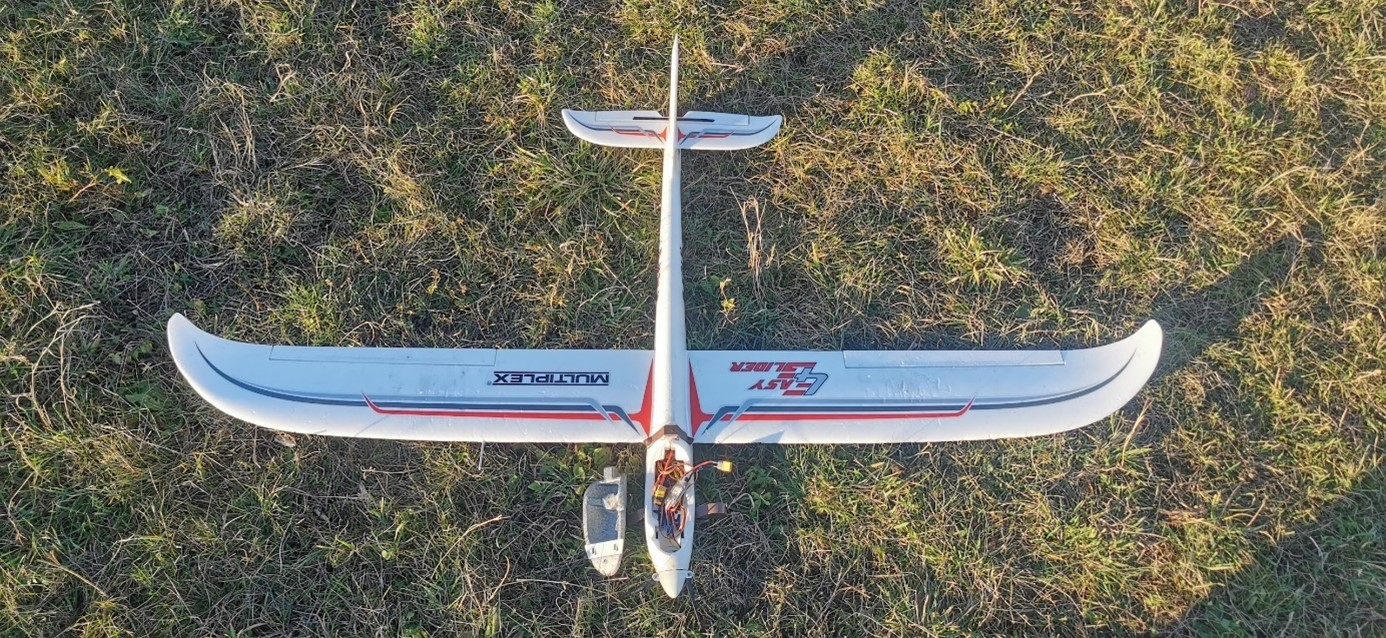
\includegraphics[width=1\textwidth]{budowa1}
    \caption{Dodać podpis :)}
\end{figure}
Samolot ten nie jest jednak przystosowany do przenoszenia większej ilości urządzeń podkładowych poza odbiornikiem i baterią. Jego mocno ograniczona objętość kadłuba sprawiała, że wymiana baterii wiązała się z każdorazowym rozłączeniem kabli oraz wyjęciem większości elektroniki. Taki proces każdorazowo związany jest z możliwością uszkodzenia elementów na płytce prototypowej, a także zajmował dużo czasu. Samolot jest także jedynie modelem służącym do testów, dlatego konieczne było zaprojektowanie i przygotowanie modelu spełniającego odpowiednie założenia wytrzymałościowe i aerodynamiczne. Model taki został zaprojektowany w programie XFLR5.
 \begin{figure}[ht]
    \centering
    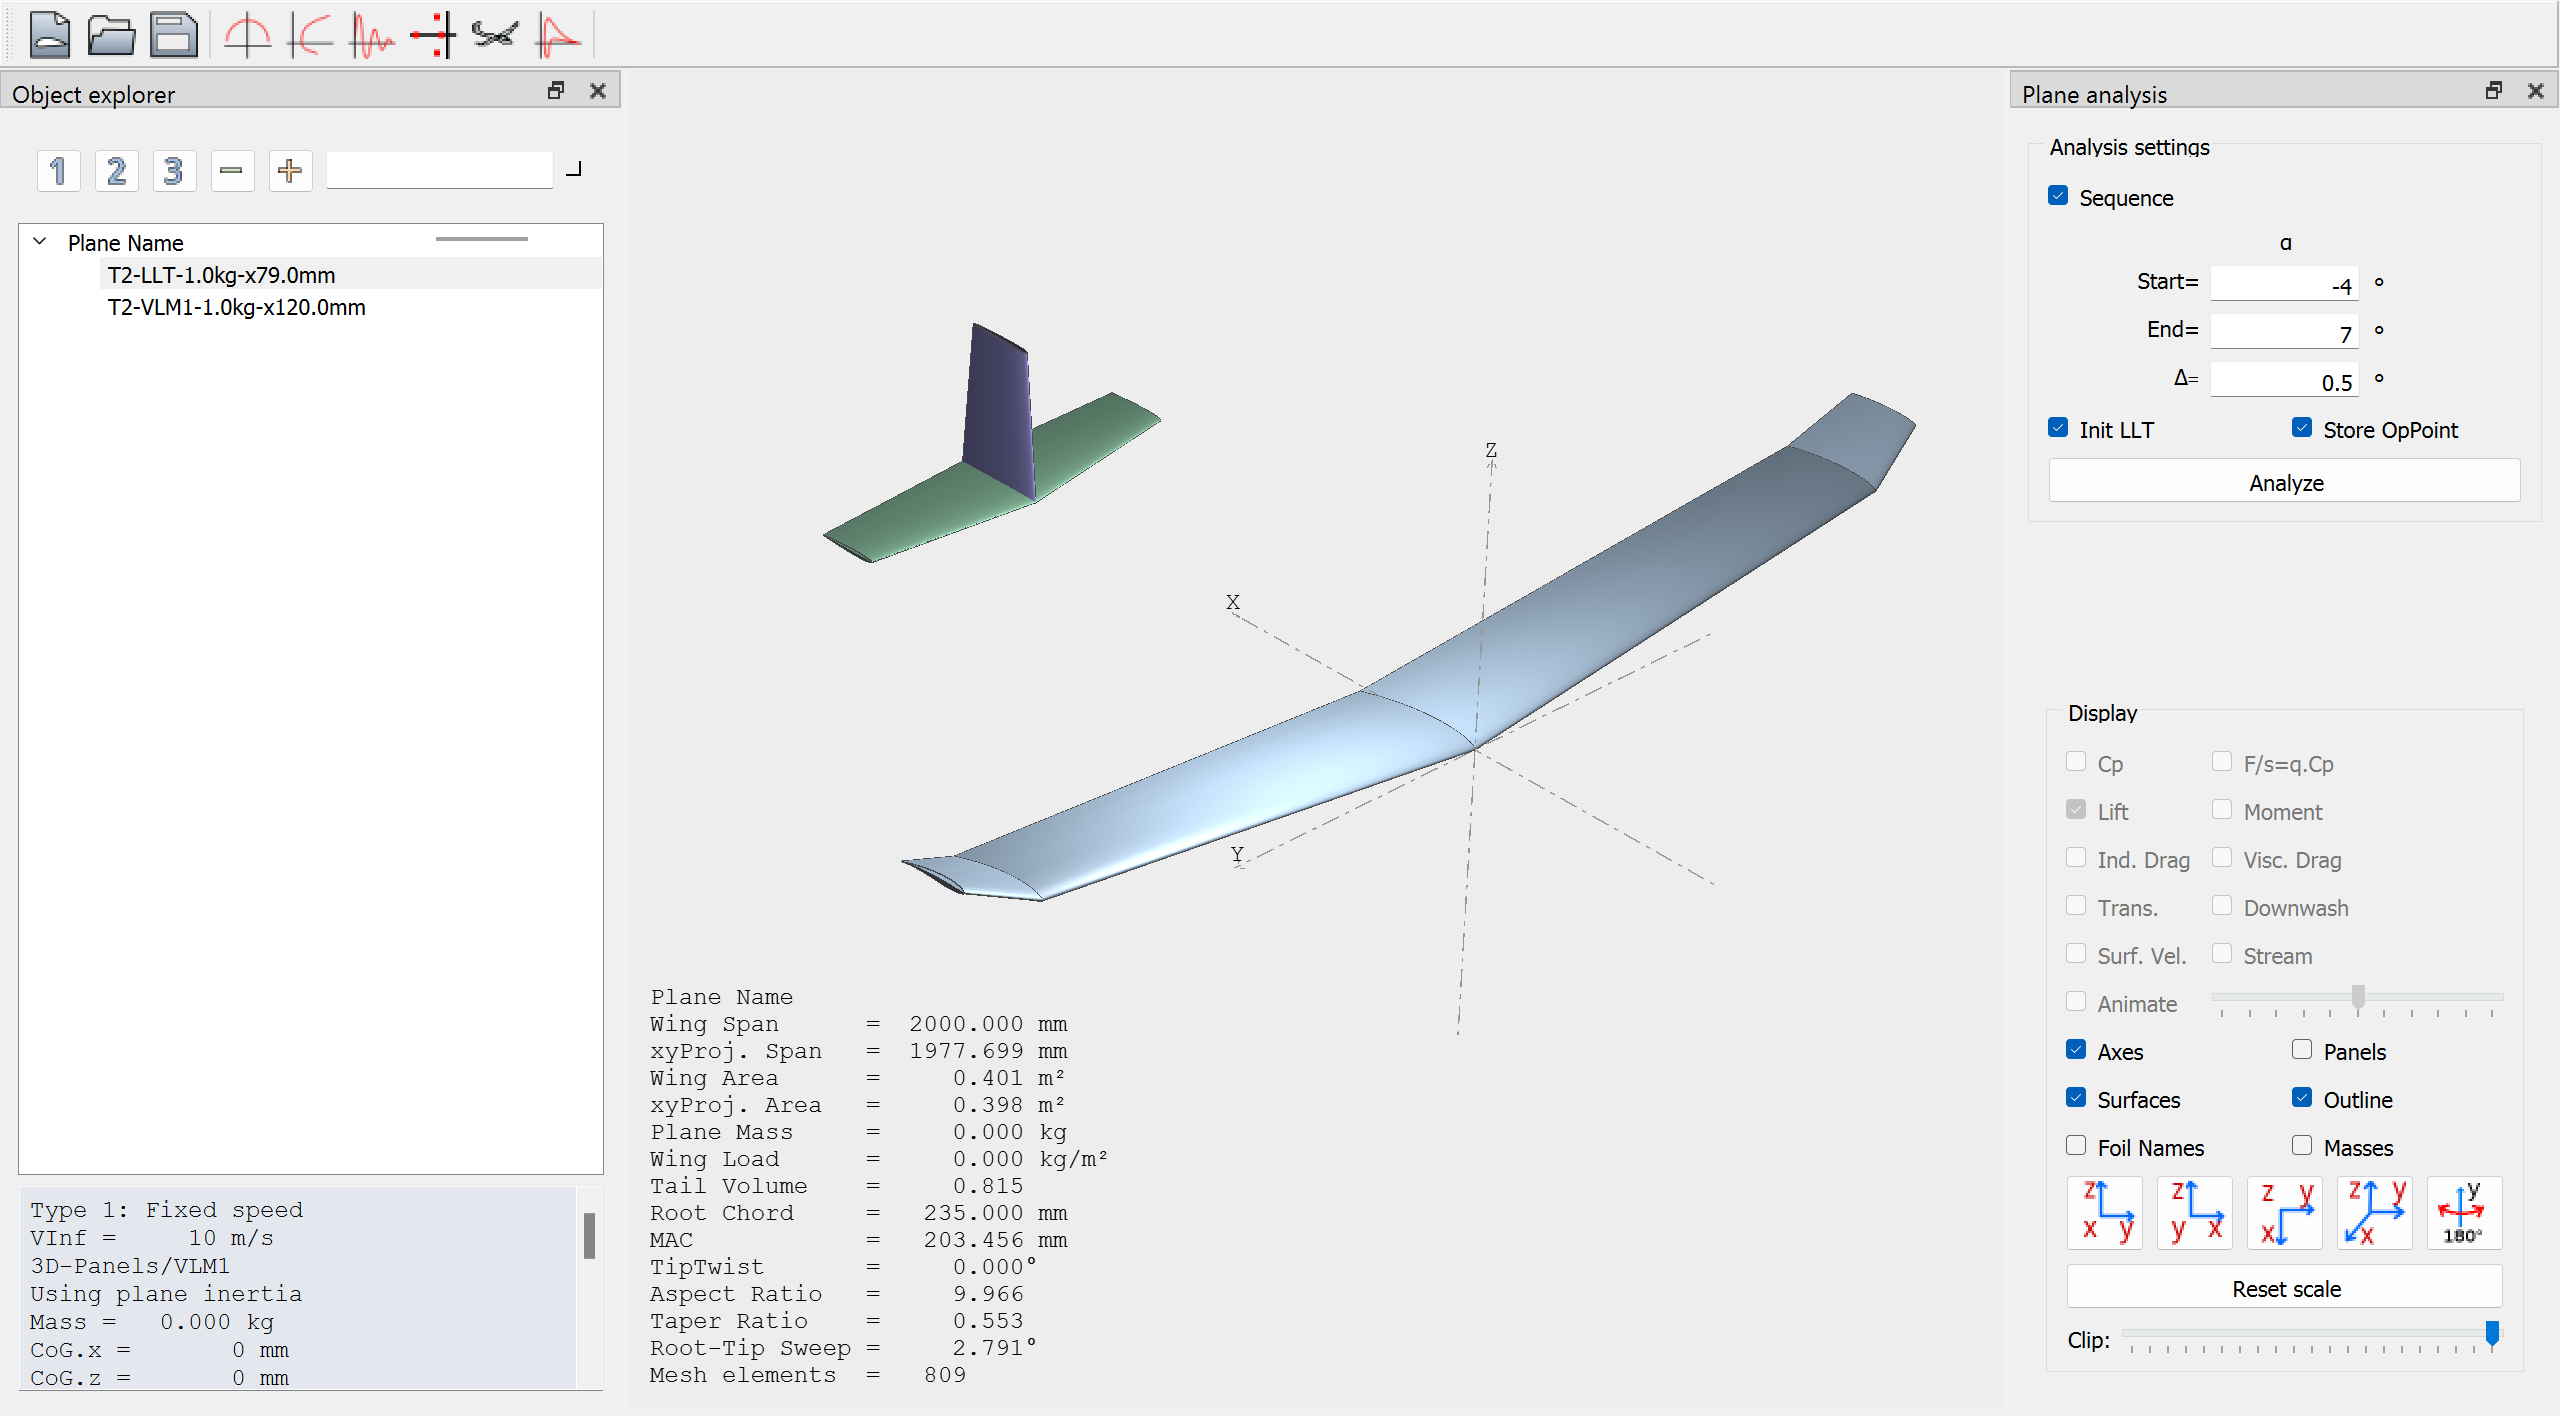
\includegraphics[width=1\textwidth]{xflr}
    \caption{Dodać podpis :)}
\end{figure}
Jako profil lotniczy skrzydła wybrany został FX 60-100. Jest on stosunkowo gruby oraz wklęsły w swojej dolnej części, co przekłada się na zwiększone opory powietrza oraz większą siłę nośną, przy równoczesnej niższej prędkości przelotowej. Na końcach skrzydeł znajdują się uszka o tym samym profilu. Kąt wzniosu skrzydeł wynosi 5º na każde skrzydło, natomiast uszka wzniesione są o dodatkowe 15 º.  Całkowita rozpiętość skrzydeł wynosi 2 metry.
 \begin{figure}[ht]
    \centering
    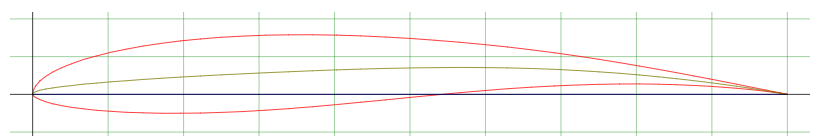
\includegraphics[width=1\textwidth]{fx60}
    \caption{Dodać podpis :)}
\end{figure}
Statecznik poziomy i pionowy posiadają profil lotniczy NACA 0008, który jest profilem symetrycznym. Statecznik jest stosunkowo duży, co zapewnia dodatkową stabilizację podczas lotu. Znajduję się on 90 cm od początku krawędzi natarcia skrzydła głównego.
 \begin{figure}[ht]
    \centering
    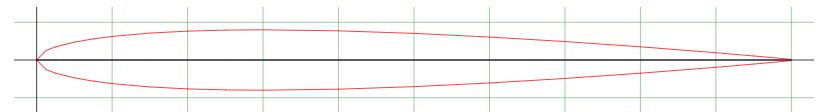
\includegraphics[width=1\textwidth]{naca0008}
    \caption{Dodać podpis :)}
\end{figure}
Coś o parametrach samolotu?
Po zakończeniu procesu projektowania, pierwszym niezbędnym elementem do przygotowania są bryty na skrzydła oraz statecznik wykonane z polistyrenu ekstrudowanego, potocznie nazywanego styrodurem. Ze styrodurowej płyty, przy pomocy plotera termicznego, za pomocą gorącego drutu wycinany jest obrys profili przez dwie oddalone od siebie karetki. W ten sposób możliwe jest otrzymanie dokładnej geometrii zaprojektowanego skrzydła, a równocześnie form negatywowych, które zostaną wykorzystane później w procesie laminowania.
\begin{figure}[ht]
    \centering
    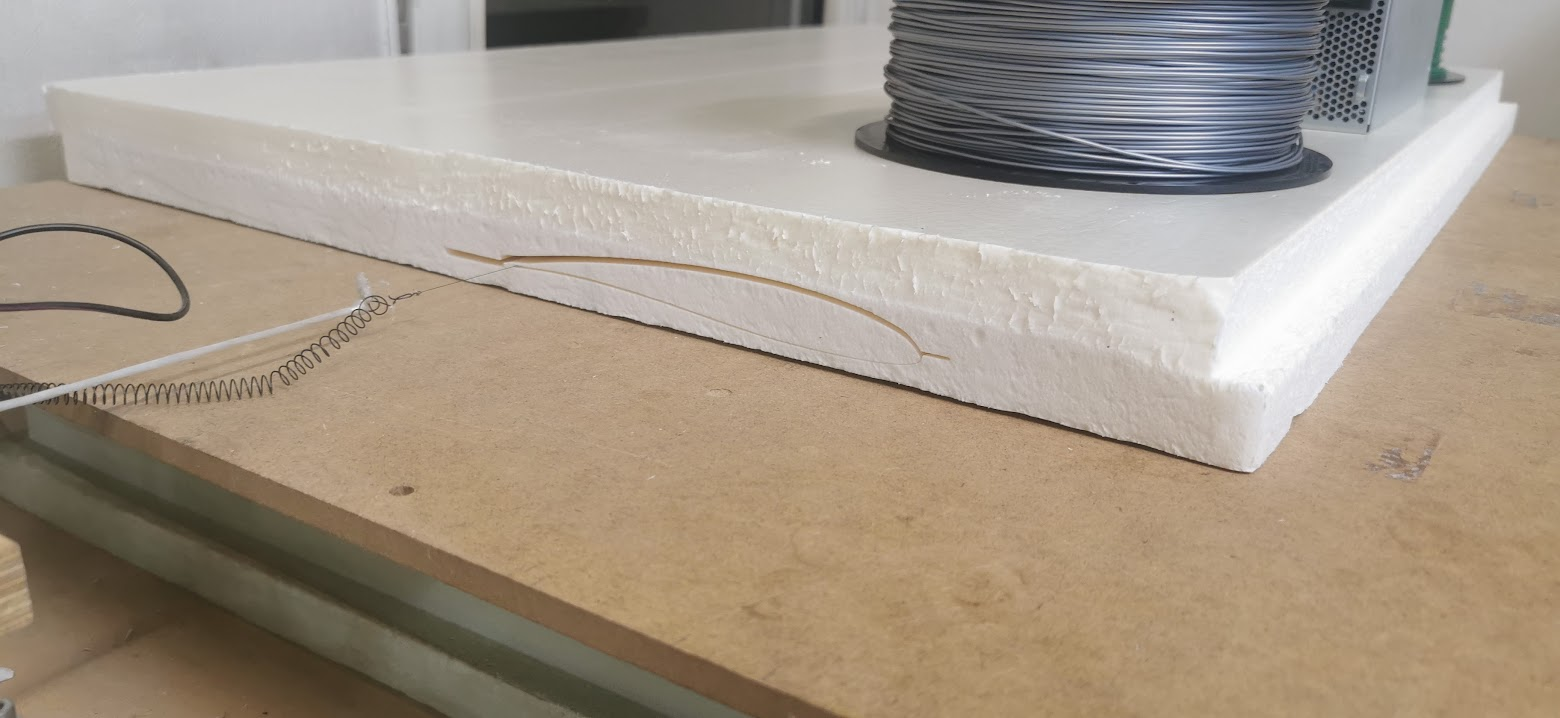
\includegraphics[width=1\textwidth]{budowa5}
    \caption{Dodać podpis :)}
\end{figure}
 
W analogiczny sposób wycięte zostały bryty na uszka oraz elementy statecznika. Przed dalszym procesem skrzydła muszą zostać okablowane, czyli przewody doprowadzające zasilanie i sygnały do różnych elementów muszą zostać umieszczone w styrodurze tak, aby nie zaburzały powierzchni profilu lotniczego. W widocznym poniżej prawym skrzydle widoczne są przewody do modułu rurki Pitota, modułu ogniw fotowoltaicznych oraz do serwomechanizmu poruszającego lotką.
 \begin{figure}[ht]
    \centering
    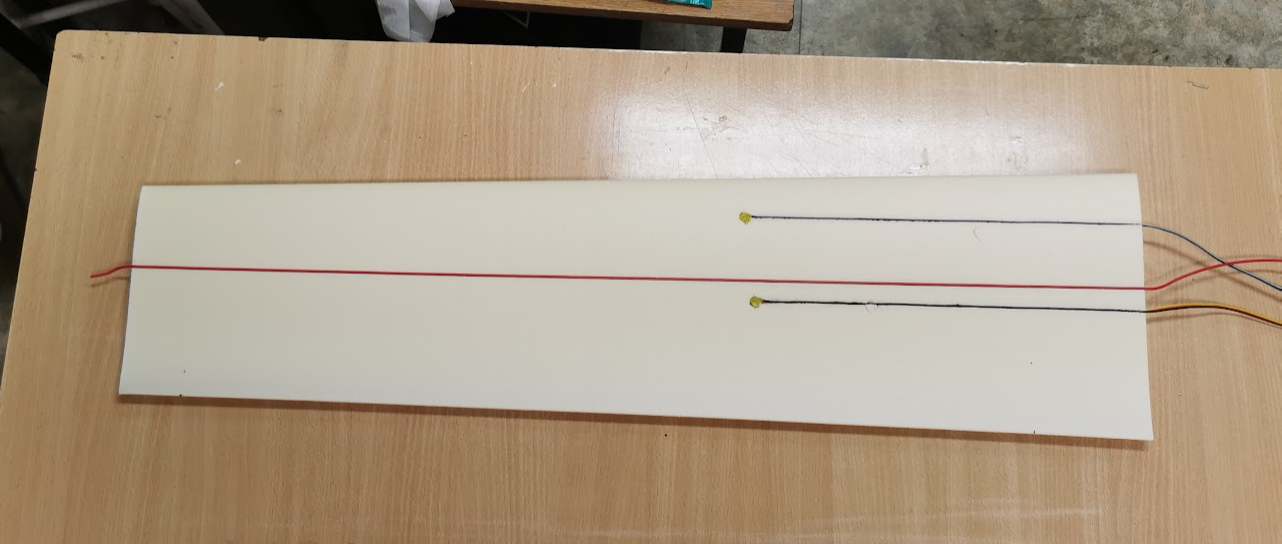
\includegraphics[width=1\textwidth]{okablowany}
    \caption{Dodać podpis :)}
\end{figure}
Same ogniwa fotowoltaiczne zostały uprzednio zalaminowane przy pomocy opracowanej przez SKN AGH Solar Plane metodzie, która pozwala na przylutowanie do siebie szeregu ogniw, a następnie zabezpieczenie ich przy pomocy folii od górnej strony oraz włókna szklanego od dołu. Dzięki temu możliwe jest następne wykorzystanie takiego modułu w procesie laminowania skrzydeł. Zapewnia to możliwość ich późniejszego dostosowania do kształtu skrzydła bez znaczącego spadku sprawności.
 \begin{figure}[ht]
    \centering
    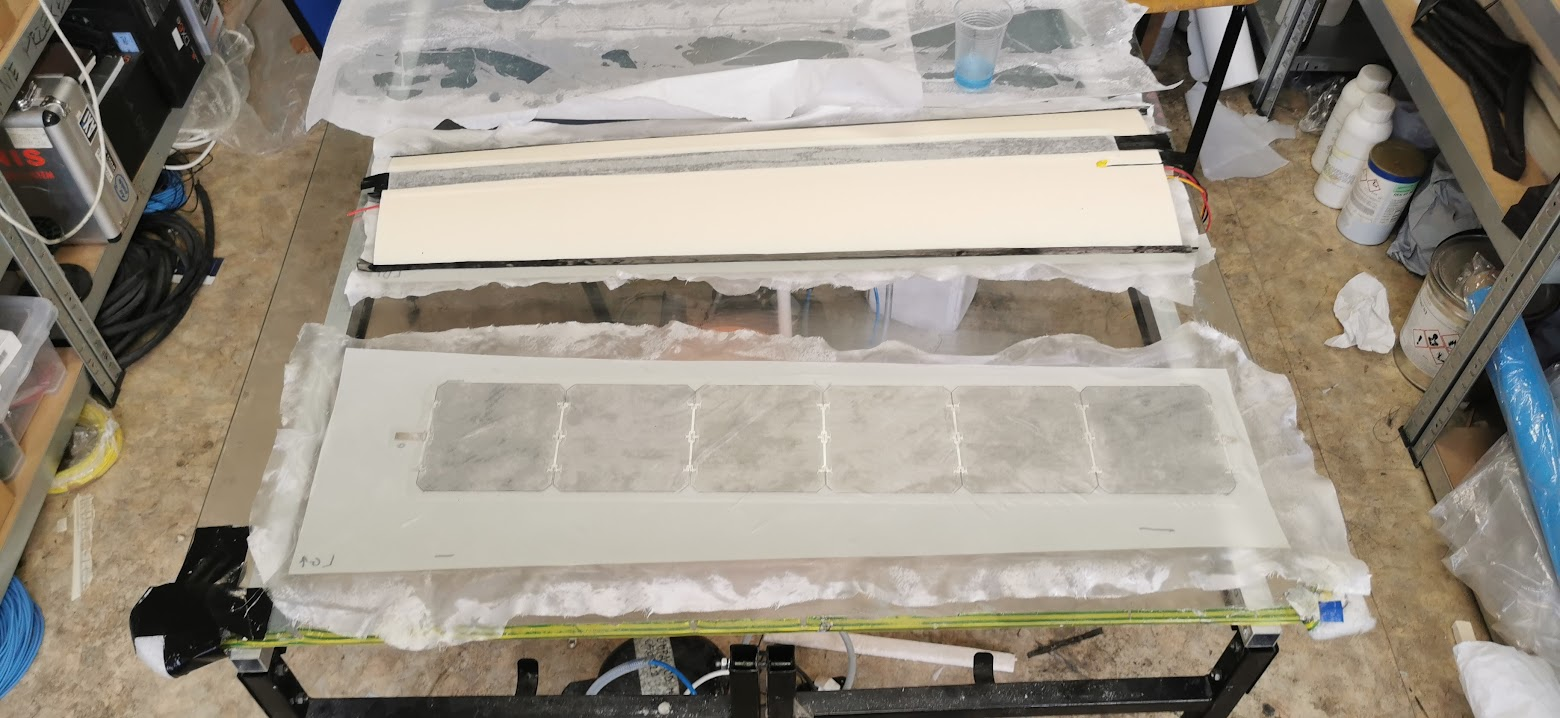
\includegraphics[width=1\textwidth]{budowa7}
    \caption{Dodać podpis :)}
\end{figure}
Skrzydła zyskują swój ostateczną formę w procesie laminowania. Polega on na odpowiednim nałożeniu warstw laminatu na bryt i nasączeniu ich żywicą epoksydową. Z uwagi na instalację fotowoltaiczną umieszczoną na skrzydłach nie jest możliwe wykorzystanie laminatu z włókna węglowego, ponieważ istnieje bardzo duże ryzyko zwarcia instalacji na całej jej długości –przez dodatkową warstwę tkaniny szklanej przebić się mogą  pojedyncze włókna węglowe, będące bardzo dobrymi przewodnikami energii elektrycznej. Jako laminat wykorzystane więc zostały dwie warstwy tkaniny szklanej o gramaturze 48 g/m2 na każdą powierzchnię. Węglowy rowing został jedynie wykorzystany jako wzmocnienie krawędzi spływu, natomiast na krawędź natarcia oraz dźwigar zostały wykonane z taśmy węglowej o szerokości 20 mm (na dźwigrze znajdują się dwa). Na gotowy laminat zostaje położona folia Mylar, która pozwala odbić idealnie gładką powierzchnię. Tak przygotowane bryty laminaty są następnie umieszczane w worku próżniowym, z którego przy pomocy pompy usuwane jest powietrze do ciśnienia -400 mbar względem atmosfery. Ciśnienie to jest stosunkowo wysokie, w tego typu procesach częściej spotykane jest uzyskanie próżni rzędu -800 do -900 mbar, jednak taki nacisk może powodować pękanie ogniw fotowoltaicznych.

Dzięki temu uzyskany jest bardzo duży, równomierny nacisk na całą powierzchnię brytu. Z uwagi na wypukło-wklęsły profil lotniczy skrzydła konieczne jest umieszczenie brytów w negatywowej formie, ponieważ worek poróżniony jest w stanie mocno naciągnąć kształt brytu. Widoczne na zdjęciu gaśnice oraz akumulatory służą jako dodatkowe obciążenie form. Czas schnięcia zastosowanej żywicy epoksydowej L285 wraz z utwardzaczem H287 wynosi około 24 godziny.
 \begin{figure}[ht]
    \centering
    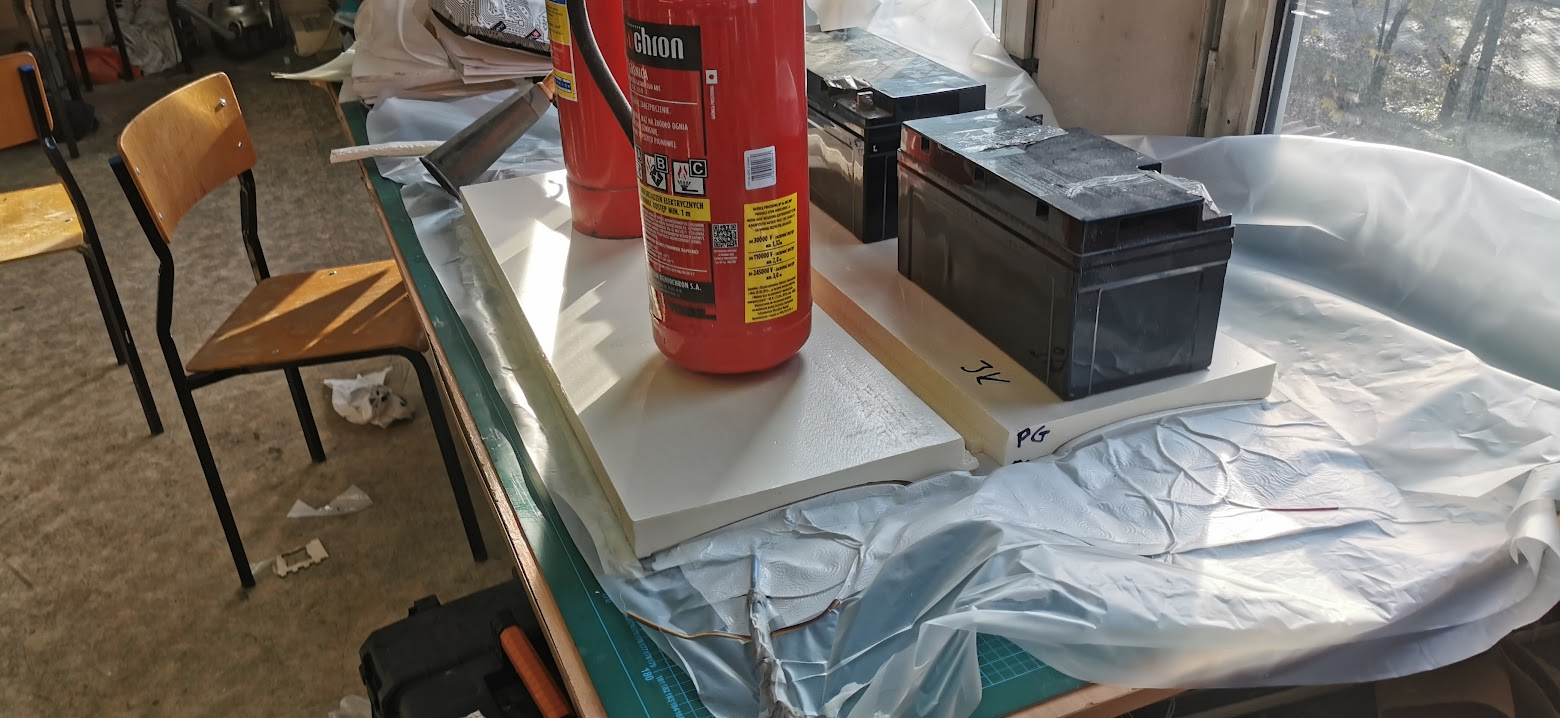
\includegraphics[width=1\textwidth]{budowa9}
    \caption{Dodać podpis :)}
\end{figure}
W analogiczny sposób zalaminowane zostały uszka oraz elementy statecznika. Przy okazji tego procesu dodatkowo wzmocniono krawędzie natarcia i spływu skrzydeł

Finalnym rezultatem procesu laminowania są widoczne na zdjęciu elementy.

Kolejnym etapem było połączenie skrzydeł oraz uszek. Efekt ten został osiągnięty przy pomocy kleju żywicznego Poxipol oraz przylaminowania fragmentów dwukierunkowej tkaniny węglowej.
 \begin{figure}[ht]
    \centering
    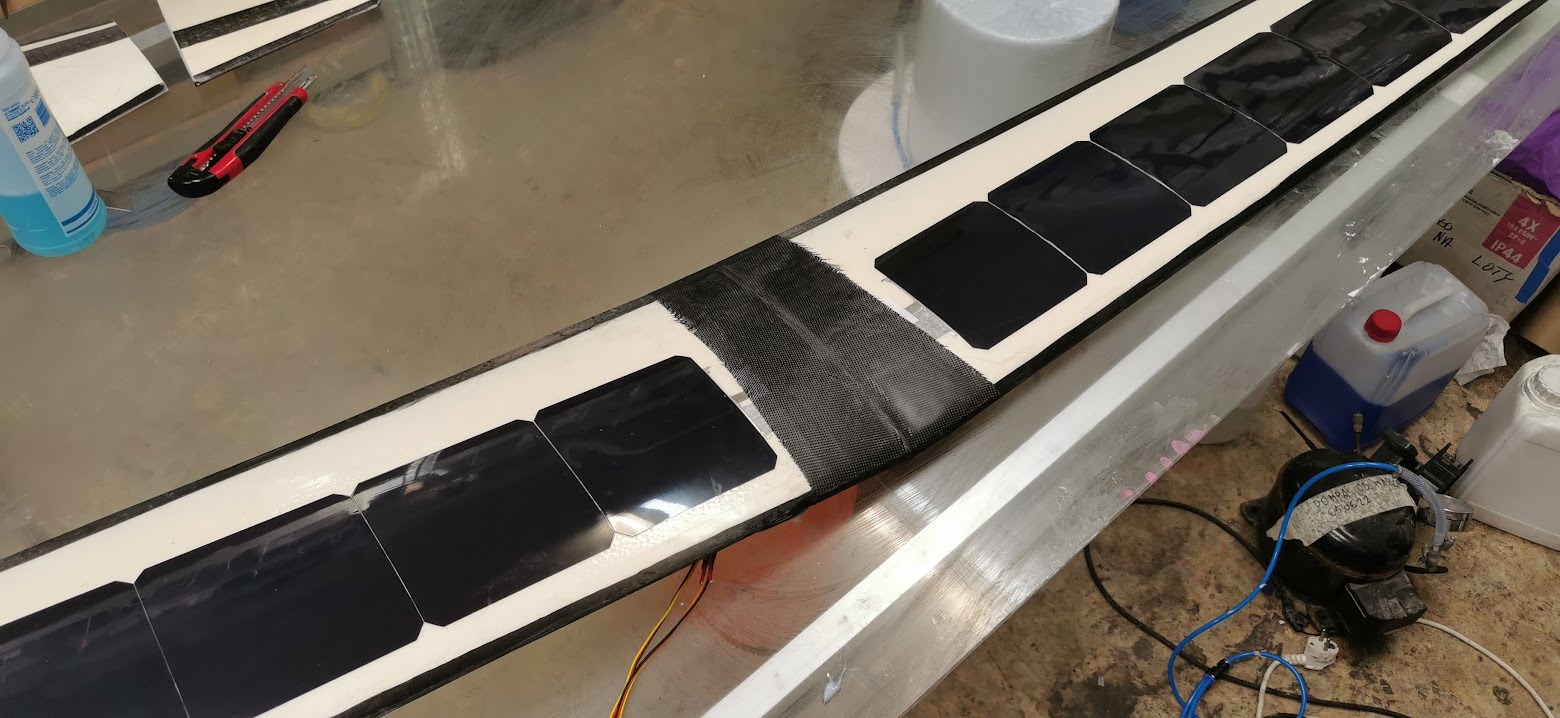
\includegraphics[width=1\textwidth]{budowa12}
    \caption{Dodać podpis :)}
\end{figure}
Elementy statecznika także zostały sklejone przy pomocy kleju Poxipol. Całość została umieszczona na rurze węglowej o długości 1m i średnicy 20mm.
 Ostatnim niezbędnym laminowanym elementem była podstawka pod skrzydła, umożliwiająca uzyskanie kąta zaklinowania skrzydeł oraz ich systemu mocowania. Podstawka została zaprojektowana w programie Fusion 360, wyfrezowana na urządzeniu CNC i finalnie zalaminowana jedną warstwą dwukierunkowej tkaniny węglowej.
Szkielet kadłuba został wykonany z list sosnowych, sklejonych ze sobą klejem cyjanoakrylowym. Wnętrze kadłuba zostało rozplanowane w taki sposób, aby umożliwić jak najwygodniejszy dostęp do modułu kontrolera oraz baterii. W skrzydłach umieszczone zostały węglowe tulejki, w których umieszczone są śruby mocujące M4, przy pomocy których skrzydła są przykręcane do kadłuba. 
 \begin{figure}[ht]
    \centering
    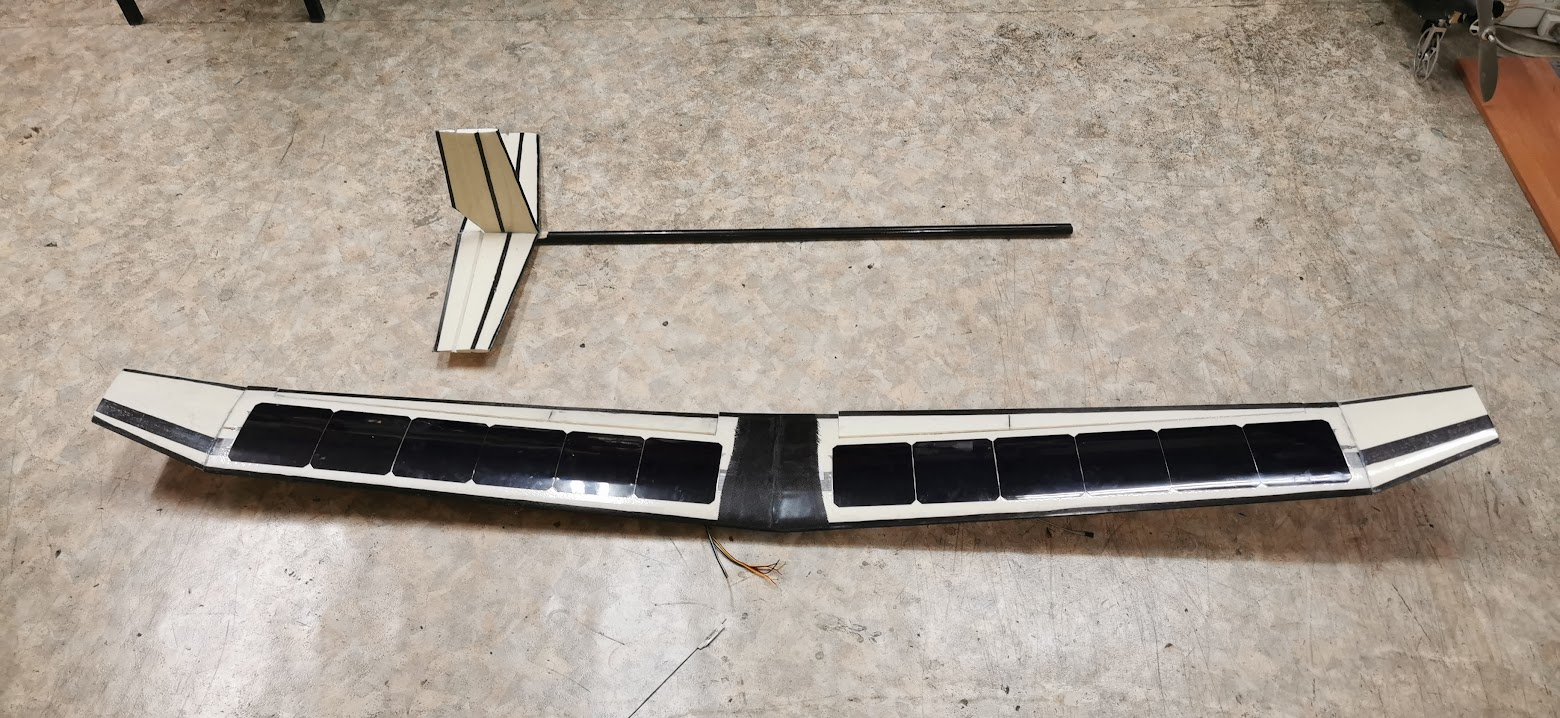
\includegraphics[width=1\textwidth]{budowa13}
    \caption{Dodać podpis :)}
\end{figure}
Stery kierunku i wysokości obsługiwane są przy pomocy serwomechanizmów umieszczonych w kadłubie oraz bowdenów umieszczonych wzdłuż rury ogonowej. We wszystkie powierzchnie sterowe wklejone zostały wykonane z płyty węglowej orczyki prowadzące. 

\begin{figure}[ht]
    \centering
    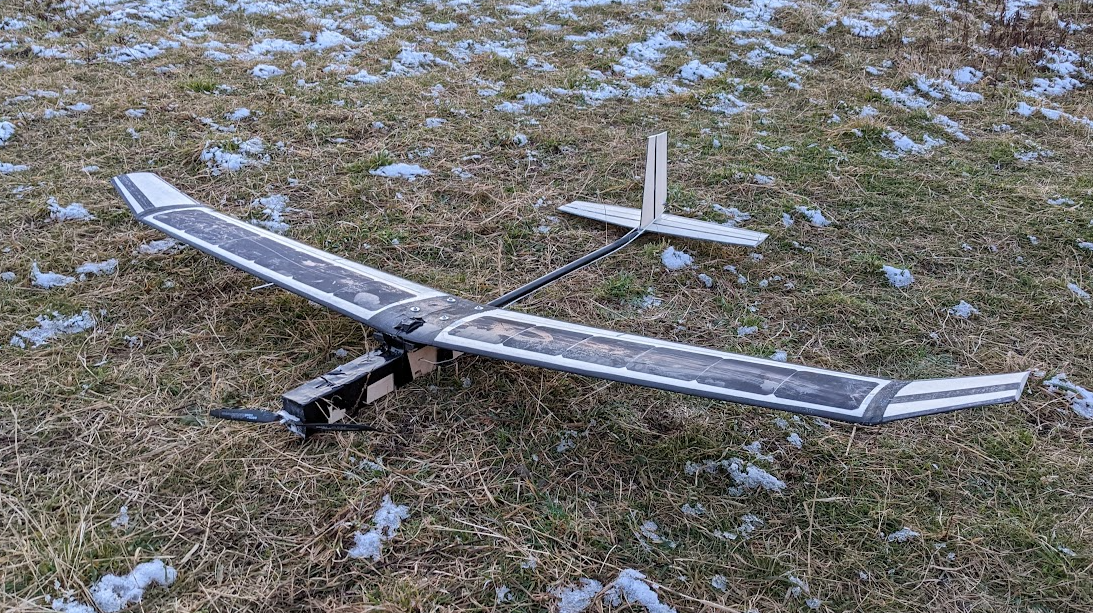
\includegraphics[width=1\textwidth]{caly}
    \caption{Dodać podpis :)}
\end{figure}
\begin{figure}[ht]
    \centering
    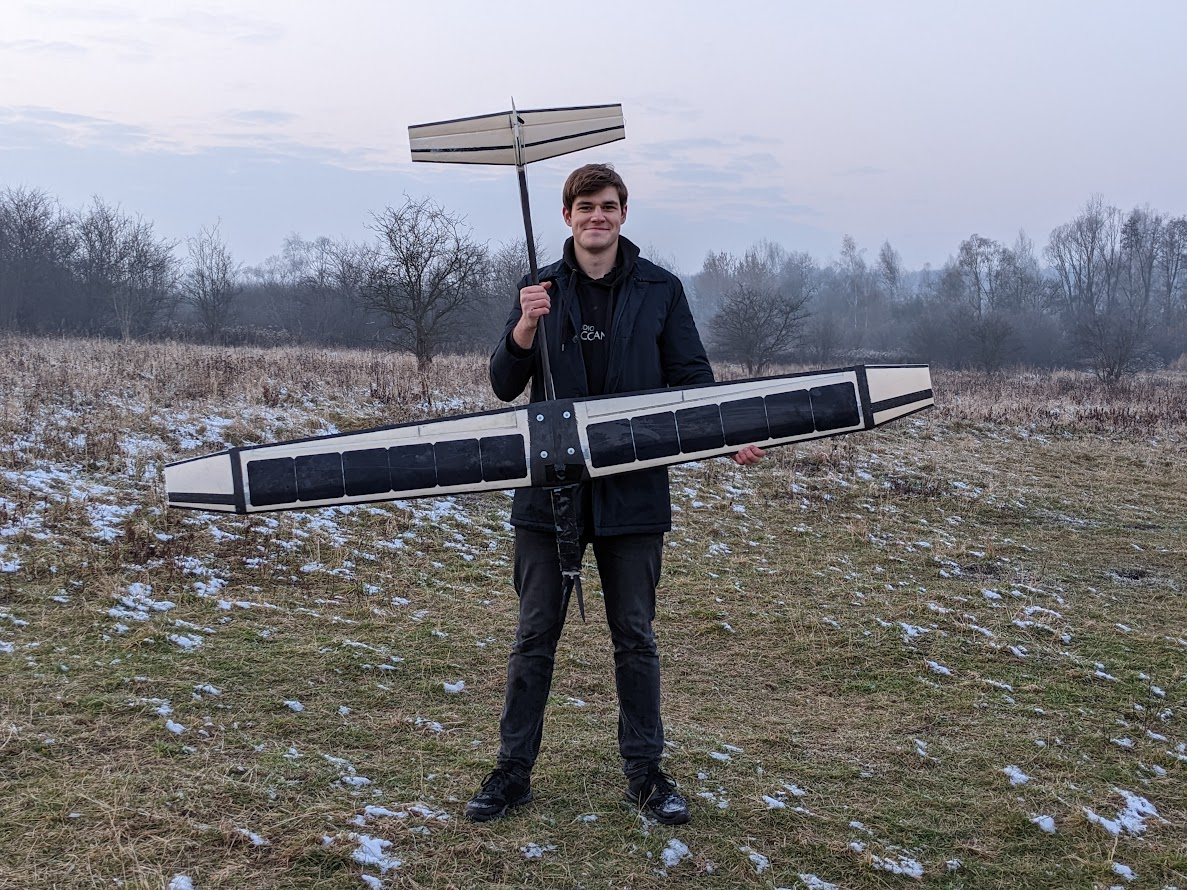
\includegraphics[width=1\textwidth]{budowa16}
    \caption{Dodać podpis :)}
\end{figure}
Po umieszczeniu całej elektroniki podkładowej, szkielet kadłuba został wzmocniony i zabezpieczony balsą modelarską. Przewidziana została możliwość szybkiego dostępu do kontrolera jak i do baterii przy pomocy umieszczonych na zawiasach zamknięciach.

 \FloatBarrier
\subsection{Moduł instalacji fotowoltaicznej}
Prace nad kontrolerem opartym o sieć neuronową wymagają zebrania ogromnej ilości danych oraz obserwacji samolotu w powietrzu, co przekłada się na konieczność utrzymania samolotu w powietrzu tak długo jak to możliwe - każde lądowanie, wymiana baterii i kalibracja zajmuje bardzo cenny podczas testów czas. Aby zmaksymalizować czas samolotu w powietrzu, na jego skrzydłach umieszczona została instalacja fotowoltaiczna, która wspomaga zasilanie z baterii lub nawet pozwala ją częściowo naładować.

Instalacja składa się z 12 ogniw SunPower gen. 4 (wymiary 125mm na 125mm), każde o znamionowej mocy 3,6W, działające przy napięciu maksymalnym 0,6V. Zostały one wybrane ze względu na wysoką sprawność sięgająca nawet 23\%, a dodatkowo możliwe jest ich kupienie w czystej, niezabezpieczonej formie. Pozwala to na umieszczenie ich na skrzydłach ze względu na grubość rzędu dziesiątej części milimetra oraz giętkość pozwalającą na dopasowanie do profilu lotniczego. Przed tym procesem konieczne jest jeszcze ich zlutowanie (na każde skrzydło wykonany został szereg 6 ogniw), a następnie odpowiednie zabezpieczenie. Odbywa się to poprzez umieszczenie warstwy folii zabezpieczającej o grubości 80$\mu$m przy pomocy strumienia gorącego powietrza. Powietrze znajdujące się pomiędzy ogniwami a folią jest uprzednio usuwane przy pomocy pompy próżniowej oraz wałeczków. Folia poza obrysem ogniw przykleja się do umieszonej pod spodem warstwy tkaniny szklanej o gramaturze 48$\frac{g}{m^2}$, która pozwala na późniejsze przyklejenie w trakcie procesu laminowania skrzydeł. 

Wszystkie 12 ogniw umieszczone na skrzydłach połączone są szeregowo, co daje panel o mocy znamionowej 43,2W. Należy wziąć jednak pod uwagę zabezpieczenie ogniwa zwykłą folią (a nie na przykład EVA) oraz zakrzywienie ogniwa na skrzydle, co znacząco wpływa na ich sprawność, dlatego rzeczywista moc układu jest niższa. Z uwagi na brak odpowiednich warunków pogodowych, do jej sprawdzenia wykorzystane zostało stanowisko badawcze.

Warto zaznaczyć, że uzyskanie instalacji o takiej mocy jest bardzo dużym sukcesem i nie było by możliwe bez setek godzin spędzonych na opracowaniu metod laminowania oraz umieszczania instalacji na skrzydłach przez SKN AGH Solar Plane.

Dzięki uprzejmości doktora inżyniera Krzysztofa Sornka z Instytutu Zrównoważonego Rozwoju Energetycznego AGH możliwe było przeprowadzenie badań gotowej instalacji na skrzydłach. Z uwagi na brak warunków pogodowych, badania zostały przeprowadzone na stanowisku badawczym, które powala na uzyskanie mocy promieniowania zbliżonej do warunków podczas słonecznego dnia w lecie na ternie Polski - około 1000$\frac{W}{m^2}$. Uzyskane jest to dzięki systemowi lamp halogenowych, które niestety bardzo szybko się nagrzewają - badania musiały być więc prowadzone bardzo sprawnie. Było to możliwe dzięki użyciu skryptu do automatycznego pomiaru wykonanego przy pomocy sztucznego obciążenia. Badanie trwało więc zaledwie kilkanaście sekund i pozwoliło uniknąć zbytniego przegrzania ogniw fotowoltaicznych. Instalacja była badana osobno na każdym skrzydle ze względu na ograniczoną powierzchnię stanowiska. Wynikiem badań było uzyskanie charakterystyk prądowo-napięciowych, w tym także generowanej mocy w zależności od napięcia.

\begin{figure}%
    \centering
    \subfloat[\centering label 1]{{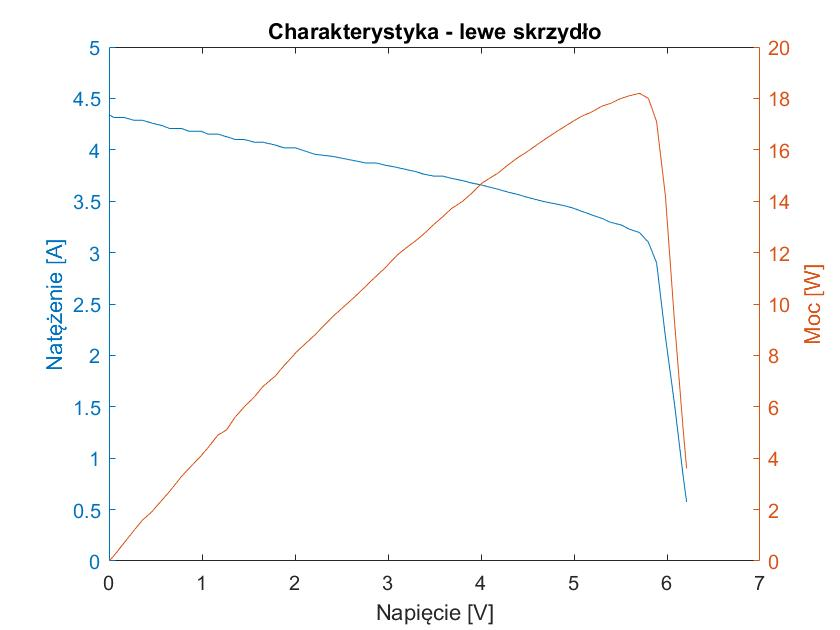
\includegraphics[width=0.45\textwidth]{leweprzetarte} }}%
    \qquad
    \subfloat[\centering label 2]{{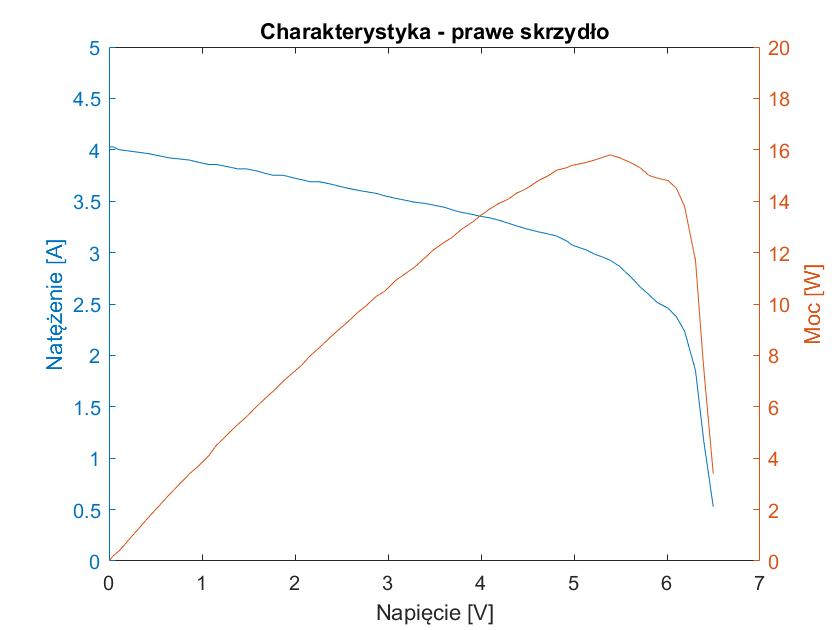
\includegraphics[width=0.45\textwidth]{praweprzetarte} }}%
    \caption{2 Figures side by side}%
    \label{fig:example}%
\end{figure}

Na wykresach charakterystyka mocy ma widoczne globalne maksimum, które nazywane jest maksymalnym punktem pracy panelu fotowoltaicznego. Stosowne byłoby zatem użycie modułu MPPT (Maximum Power Point Tracker), który pozwala na dostosowanie zależności napięcia i naprężenia w taki sposób, aby uzyskiwać maksymalną moc. Niestety, takie moduły dostępne na rynku są dostosowane do znacznie większych instalacji, a ich wymiary i waga nie pozwalają na użycie w samolocie. Prace nad autorskim modułem zajęły by zbyt dużo czasu dlatego najlepszym rozwiązaniem jest użycie odpowiednio dobranej przetwornicy z rodziny step-up. Przy tak małej instalacji, różnica między użyciem przetwornicy a modułu MPPT jest bardzo mała, ponadto przetwornica pracuje w trybie ciągłym, komercyjne moduły MPPT potrzebują czasu liczonego w sekundach na ustawienie się. Zgodnie z założeniem projektowym samolot będzie wykonywał dużą ilość manewrów, zmieniając cały czas kąt nachylenia ogniw względem słońca, zatem przetwornica jest znacznie efektywnijszym rozwiązaniem. Wybranym modułem został Pololu U3V50AHV, pracujący z natężeniem do 5A i napięciem 3-30V. Przetwornica została ustawiona na napięcie wyjściowe 12,6V, co odpowiada maksymalnemu napięciu używanego akumulatora Li-Po 3S. Dzięki temu, w przypadku zużycia mniejszej ilości energii przez samolot niż jest w stanie wyprodukować instalacja fotowoltaiczna, nadmiar energii zostanie wykorzystany do ładowania pakietu baterii.

Dodatkowym eksperymentem przeprowadzonym podczas badań było także sprawdzenie wpływu zabrudzenia na instalacji fotowoltaicznej na jej sprawność. Niestety okazało się, że różnica ta nie jest możliwa do wykrycia przy użyciu stanowiska badawczego tego typu - większy wpływ na wyniki miał stopień rozgrzania lamp czy delikatnie inne ustawienie skrzydła na stole roboczym.

\begin{figure}%
    \centering
    \subfloat[\centering label 1]{{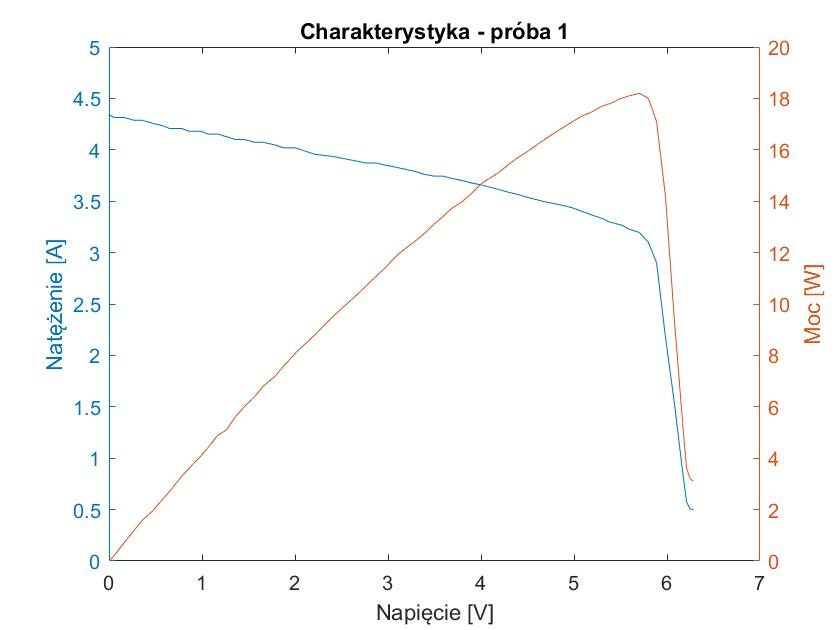
\includegraphics[width=0.45\textwidth]{porownanie1} }}%
    \qquad
    \subfloat[\centering label 2]{{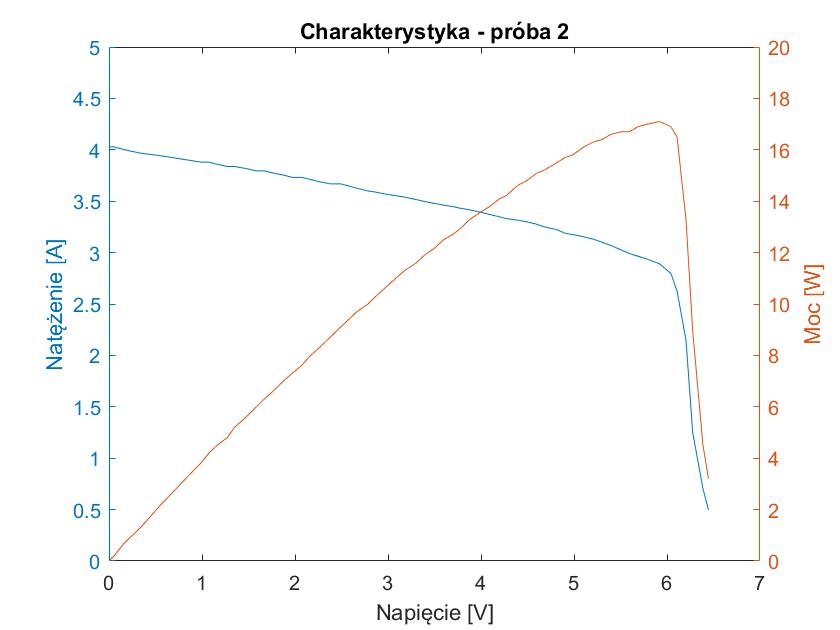
\includegraphics[width=0.45\textwidth]{porownanie2} }}%
    \caption{2 Figures side by side}%
    \label{fig:example}%
\end{figure}

Mimo krótkiego czasu wykonywania pomiarów, halogenowe lampy wytwarzają bardzo dużą ilość ciepła, co przekłada się na spadek sprawności modułów fotowoltaicznych. Widoczne jest to nawet na pomiarach wykonanych w odstępie kilkunastu sekund, gdzie różnica maksymalnej mocy wynosi około 5\%. 

Ostatnim wykonanym badaniem była analiza ogniw przy pomocy specjalistycznej kamery termowizyjnej. Podanie napięcia na końce panelu skutkuje stopniowym ogrzewaniem się ogniw. Dzięki tej technice możliwe jest wykrycie uszkodzeń powstałych w procesie laminowania ogniw lub skrzydeł. Miejsca uszkodzone stawiają większy opór elektryczny, a co za tym idzie wytwarzają więcej ciepła przy przepływie energii elektrycznej. A badaniu podano wykorzystano napięcie i natężenie znamionowe ogniw, a różnice w temperaturach sięgały kilku stopni Celsujasza. Zaobserwowano znacznie większe uszkodzenia szeregu ogniw na prawym skrzydle, co możne tłumaczyć różnicę koło 10\% maksymalnej mocy.

\FloatBarrier
\subsection{Moduł kontrolera lotu}
Pierwszym krokiem podczas pracy nad projektem  było przygotowanie listy parametrów, które są brane pod uwagę przez pilota podczas zdalnego terowania modelem. Są to: wysokość, rotacja, prędkość względem ziemi, prędkość względem wiatru, położenie samolotu, kierunek dalszej planowanej trasy. Wszystkie te wymienione elementy muszą w analogiczny sposób być brane pod uwagę przez autonomiczną jednostkę sterującą, a zbierane muszą być przy pomocy sensorów i czujników umieszczonych na pokładzie samolotu. Jednym z kluczowych założeń takiego modułu jest jego nieprzerwane, niezatrzymane i nieopóźnione działanie w podczas pracy. Utrata kontroli nad samolotem oznacza niemal pewne uderzenie w ziemię w ciągu zaledwie kilku sekund. Dlatego jako główny komputer pokładowy został wybrany mikrokontroler Teensy 4.0. Dysponuje on mikroprocesorem ARM Cortex-M7, taktowanym w trybie standardowym z częstotliwością 600 MHz. Jego innymi istotnymi zaletami jest możliwość generowania sygnału PWM przez większość wyjść cyfrowych, duża pojemność pamięci Flash (1984K) oraz RAM (1024 KB), 7 portów szeregowych UART, a także możliwość programowania w środowisku Arduino IDE (z rozszerzeniem Teensyduino). Ta ostatnia cecha jest o tyle ważna, że pozwala na użycie bibliotek do sensorów, które są najczęściej przygotowane właśnie pod tą platformę. Ich migracja na inne technologie mogła by być problematyczna. Warto zauważyć, że teoretycznie jeszcze lepszymi parametrami cechują się moduły komputerów jednopłytkowych (ang. single-board computer) jak na przykład Raspberry Pi Zero W, na którym można uruchomić system Raspbian z rodziny UNIX. Uruchomienie programu kontrolera na takim mikrokomputerze byłoby prawdopodobnie software’owo stabilniejsze i pozwalało na łatwiejsze zarządzanie wyjątkami i błędami, jednakże w przypadku zawieszenia się systemu operacyjnego lub jakiegokolwiek innego czynnika mogącego przerwać płynność działania programu bardzo prawdopodobne jest utracenie kontroli nad samolotem. Dodatkowo, system operacyjny uruchamia się w najlepszym czasie około kilkunastu sekund, co w przypadku nieplanowanego restartu w powietrzu wywołanego na przykład chwilowym spadkiem napięcia na przetwornicy oznacza pewne rozbicie modelu. Teensy uruchamia się w czasie bliskim sekundy, dodatkowo przed inicjalizacją czujników (mogącą trwać 2-3 sekundy) program sprawdza w pamięci EEPROM czy samolot nie został uprzednio uzbrojony. Jeżeli tak, czujniki pozostają wyłączone, natomiast samolot przechodzi w awaryjny tryb manualny. To rozwiązanie zapewnia samolotowi najwyższe bezpieczeństwo.
Pierwszy prototyp projektu wykorzystywał następujące moduły:
1.	Mikrokontroler Teensy 3.2
2.	Czujnik AltIMU v10
3.	Odbiornik Spectrum DSMX DX6
4.	Moduł GPS SparkFun NEO-M9N
5.	Moduł karty microSD
Całość umieszczona była we fragmencie pianki ochronnej i miało posłużyć do pierwszego sprawdzenia działania systemu. Mikrokontroler miał za zadanie gromadzić dane z czujników oraz odbierać sygnał od aparatury sterującej. W skład elektroniki pokładowej wchodziły też cztery serwomechanizmy sterujące powierzchnymi sterowymi (lotki, stery kierunki i wysokości), bezszczotkowy silnik, regulator prędkości (ESC) oraz pakiet baterii LiPo 2600mAh, który pozwalał na kilkanaście minut lotu. W module ESC znajduje się przetwornica typu UBEC 5V, która służyła jako źródło zasilania układu.
 
Wraz z kolejnymi etapami prac moduł karty microSD został zastąpiony przez moduł radiowy HC-12 operujący na częstotliwości 433 MHz. Wysyłanie danych w czasie rzeczywistym oraz ich zapis po stronie stacji odbiorczej okazał się bardziej praktycznym rozwiązaniem. Czujnik AltIMU v10, w skład którego wchodzi żyroskop, akcelerometr, magnetometr oraz wysokościomierz ciśnieniowy, okazał się działać nieprawidłowo. Został wymieniony na znacznie precyzyjniejszy moduł SparkFun ICM 20948. Dzięki wbudowanemu w bibliotekę algorytmowi DMP (InvenSense Digital Motion Processor) jest on w stanie z niesamowitą precyzją podać kąty Eulera rotacji (roll, pitch, yaw) oraz dokonywać autokalibracji podczas działania. Ma on niestety również wady: potrzebuje stosunkowo dużej ilości mocy obliczeniowej do działania oraz wysokiego taktowania procesora (producent zaleca co najmniej 100 MHz), jego poprawne działanie wymaga znacznie trudniejszej implementacji oprogramowania, a także nie jest w stanie wskazać bezwzględnego położenia w osi yaw, zatem przed każdym startem należy skalibrować go ręcznie. Czujnik rotacji jest jednym z kluczowych elementów kontrolera lotu i bardzo kluczowa jest jego powtarzalność i precyzja działania, wybrany moduł firmy SparkFun spełnia wyznaczone kryteria, a brakujący czujnik wysokościomierza został zastąpiony zewnętrznym modułem LPS25HB. Teensy 3.2 zostało zastąpione przez Teensy 4.0 z powodu lepszych parametrów oraz kompatybilności sprzętowej z biblioteką TensorflowLite.
Po ostatecznym wyborze modułów przygotowana została druga wersja urządzenia, wraz  z testową płytką PCB. Jej projekt wykonany został w programie KiCAD, i miał zapewnić stabilną pracę urządzenia oraz wymiary umożliwiające wkładanie go do samolotu testowego EasyGlider. 
 \begin{figure}[ht]
    \centering
    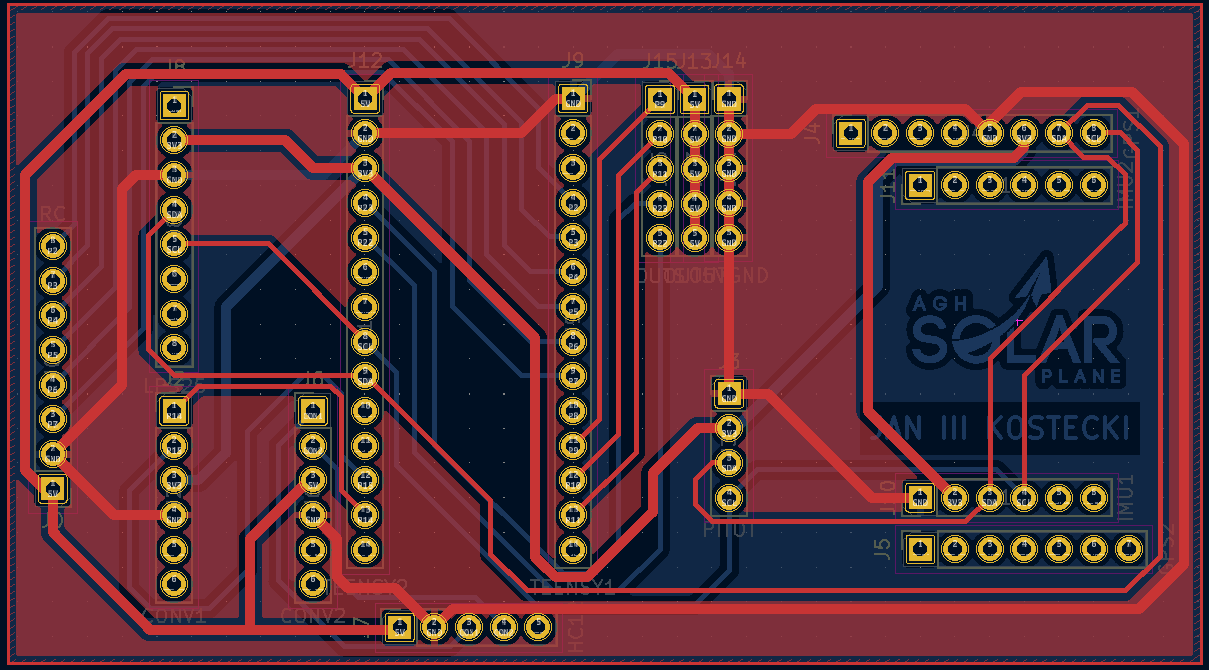
\includegraphics[width=1\textwidth]{plytkastara}
    \caption{A nice plot.}
\end{figure}
Przygotowany projekt zakładał wykonanie dwustronnej płytki PCB o wymiarach 90mm na 50mm. Wykonana została przy pomocy termotransferu tonera na specjalny laminat o grubości 1.5mm. Następnie niepotrzebna miedź została rozpuszczona w roztworze Nadsiarczanu Sodu. 
  \begin{figure}[ht]
    \centering
    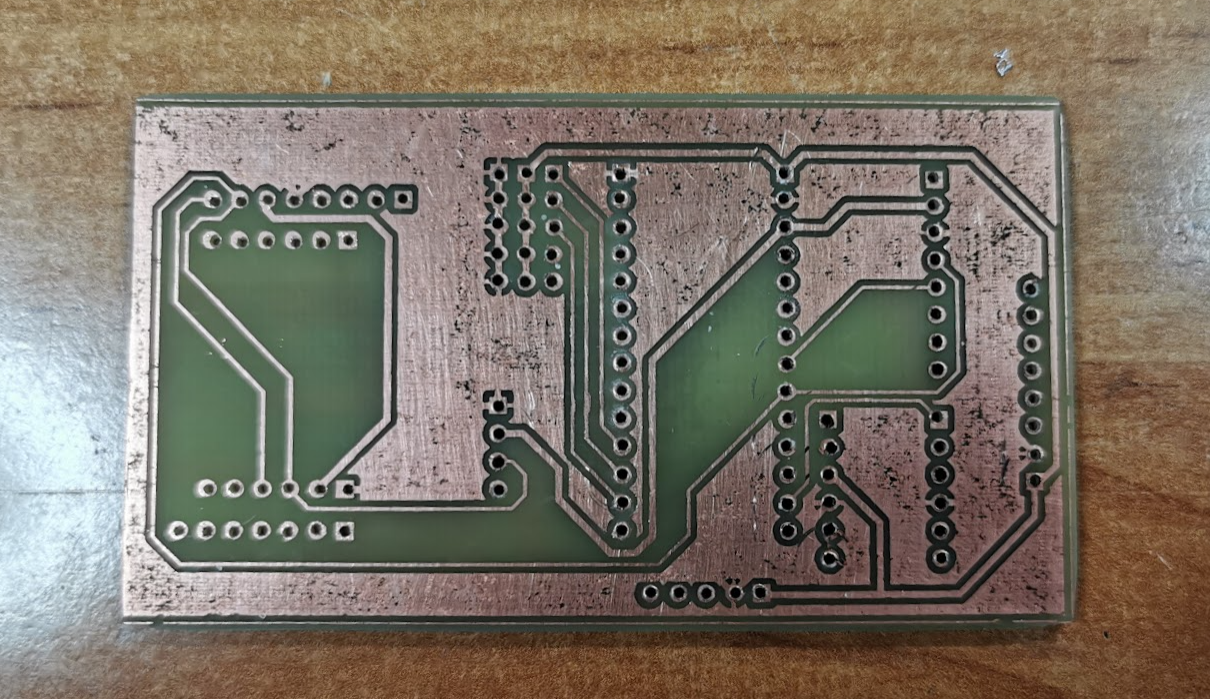
\includegraphics[width=1\textwidth]{pcb}
    \caption{A nice plot.}
\end{figure}
Aby zapewnić możliwość wymiany modułów, do gotowej płytki przylutowane zostały gniazda typu goldpin raster 2.54mm, które są kompatybilne ze wszystkimi wykorzystanymi modułami i pozwalają na szybkie przyłączanie oraz odłączanie. 
   \begin{figure}[ht]
    \centering
    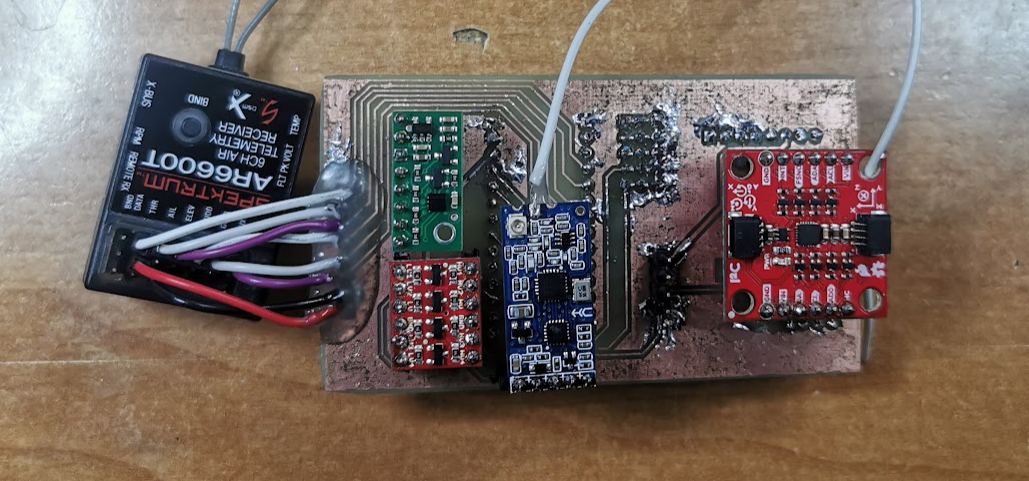
\includegraphics[width=1\textwidth]{kontorolerstary}
    \caption{A nice plot.}
\end{figure}
Po pierwszych próbach modułu w trakcie lotu okazało się, że czujnik wysokości zwraca bardzo niedokładne wyniki. Po dokładniejszej analizie okazało się, że sam czujnik działa poprawnie, jednak przez ruch silnika i śmigieł oraz pęd powietrza przelatującego przez kadłub samolotu, wyniki te są bardzo rozbieżne. Dużo bardziej precyzyjny okazał się pomiar wysokości przy pomocy modułu GPS i na jego podstawie opierane były dalsze obliczenia. 
\begin{figure}[ht]
    \centering
    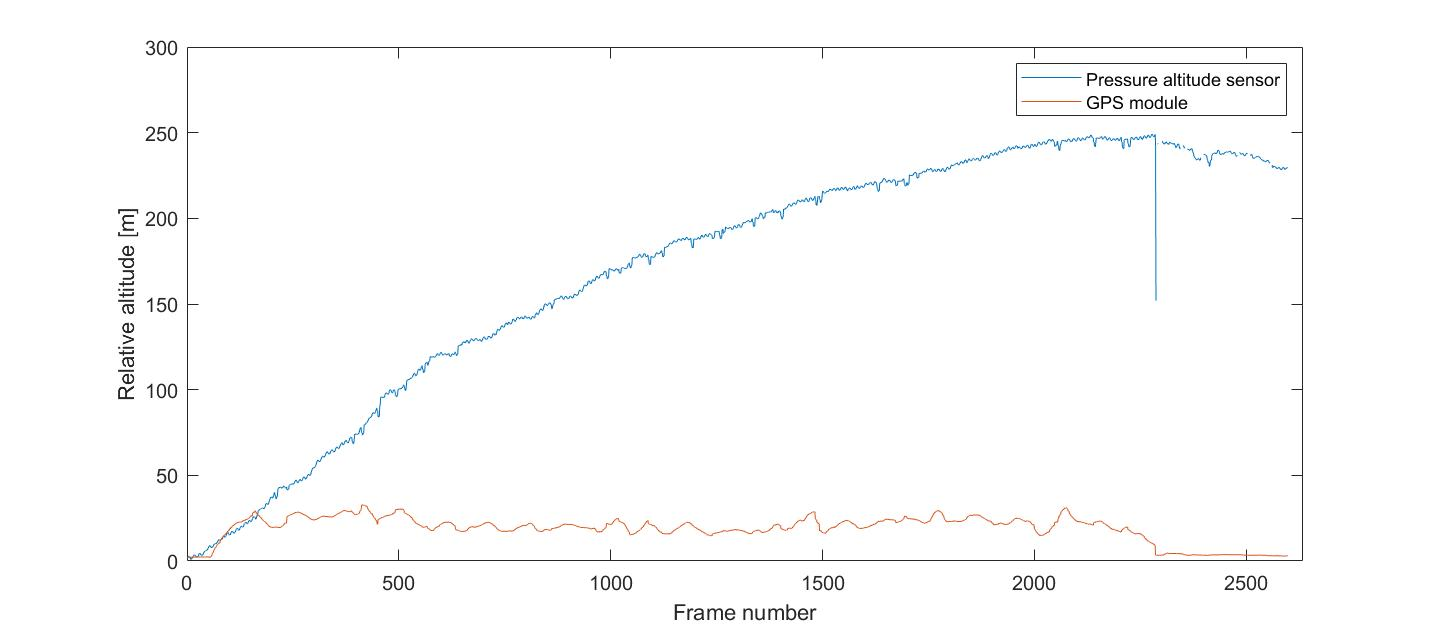
\includegraphics[width=1\textwidth]{alti}
    \caption{A nice plot.}
\end{figure}
Warto zauważyć, że widoczna na zdjęciu płytka miała charakter prototypowy, stąd widoczne niedoskonałości wykonania oraz ślady wprowadzanych poprawek. Po ustaleniu ostatecznej listy komponentów oraz skonstruowaniu dedykowanego samolotu, zaprojektowana została ostateczna wersja modułu kontrolera. Na płytce PCB wszystkie moduły zostały umieszczone po jednej stronie, zmieniony został także sposób podłączenia do układu w samolocie – ręczne wpinanie kabli do serw, ESC oraz rurki Pitota zostało zastąpione jednym gniazdem, które przy okazji pełni rolę mocowania. Z uwagi na ograniczenia czasowe projektu, wywiercone otwory nie zostały zmetalizowane, sygnał przekazywany jest między warstwami za pomocą przelotek.
   \begin{figure}[ht]
    \centering
    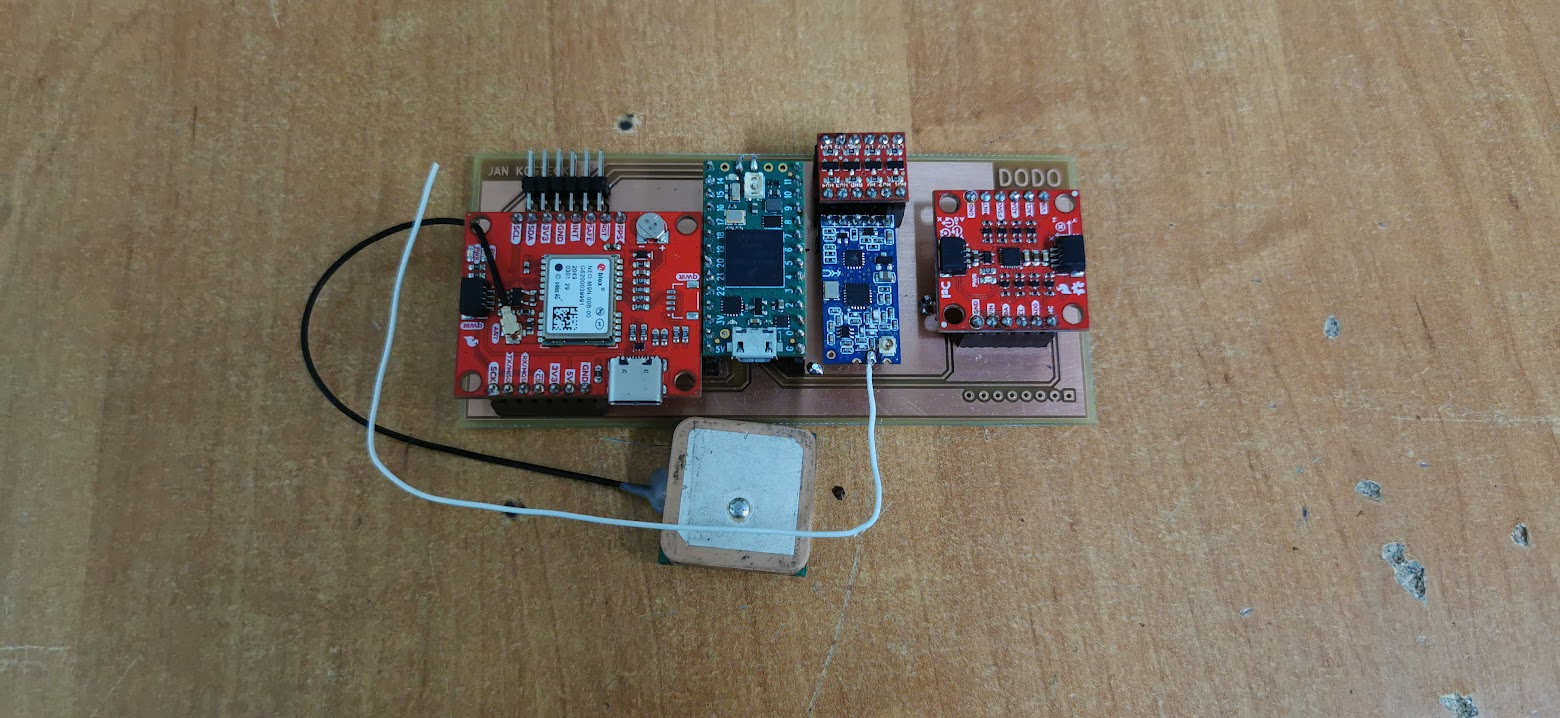
\includegraphics[width=1\textwidth]{dodokontroler}
    \caption{A nice plot.}
\end{figure}

W skład elektorniki podkładowej samolotu wchodzą także serwomechanizmy do poruszania powierzchniami sterowymi samolotu. Z uwagi na rozmiar powierzchni sterowych, wybrane zostały serwomechanizmy GO-17 MG firmy Pelikan. Posiadają one moment obrotowy od 2,2$\frac{kg}{cm}$ przy napięciu zasilającym 4,8V do nawet 2,5$\frac{kg}{cm}$ przy napięciu 6V (w samolocie napięcie zasilające za przetwornicą wynosi znamionowo 5V, w praktyce ta wartość waha się w zakresie 5V-5.5V). Silnik napędzający samolot umieszczony jest w przedniej części kadłuba, razem z elektronicznym regulatorem prędkości ESC. Wybranym modelem został Dualsky Ecko V2 2814 970kV. Jego chwilowa moc maksymalna wynosi nawet do 400W, przy obciążeniu prądowym 33A. Zgodnie z zaleceniem producenta, dobrane do niego zostały śmigła  11x7. 

 \clearpage
\subsection{Oprogramowanie kontrolera lotu}
Ciągłość pracy kontrolera jest jednym z najważniejszych założeń projektowych – jak już zostało podkreślone, jakikolwiek przestój w pracy może się wiązać z utraceniem modelu. Całe oprogramowanie znajduje się na mikrokontrolerze Teensy 4.0. Po uruchomieniu, pierwszą czynnością jest inicjalizacja:
1.	Portów szeregowych do komunikacji
2.	Serwomechanizmów 
3.	Biblioteki odczytującej dane z odbiornika
4.	Odczytanie wartości stanu uzbrojenia silnika z pamięci EEPROM
Jeżeli silnik został uzbrojony (włączony z poziomu oprogramowania) oznacza to, że samolot najprawdopodobniej znajduje się w powietrzu, dlatego od razu uruchamiany jest tryb awaryjny, aby pilot miał szanse uratować model. W innym przypadku inicjalizowane są czujniki IMU oraz GPS.

Oprogramowanie ma pozwolić na dwa tryby lotu – manualny oraz autonomiczny. W pierwszym z nich dane z czujników nie mają wpływu na lot, sygnał z aparatury jest przekazywany bezpośrednio na wyjścia.
 
    \begin{figure}[ht]
    \centering
    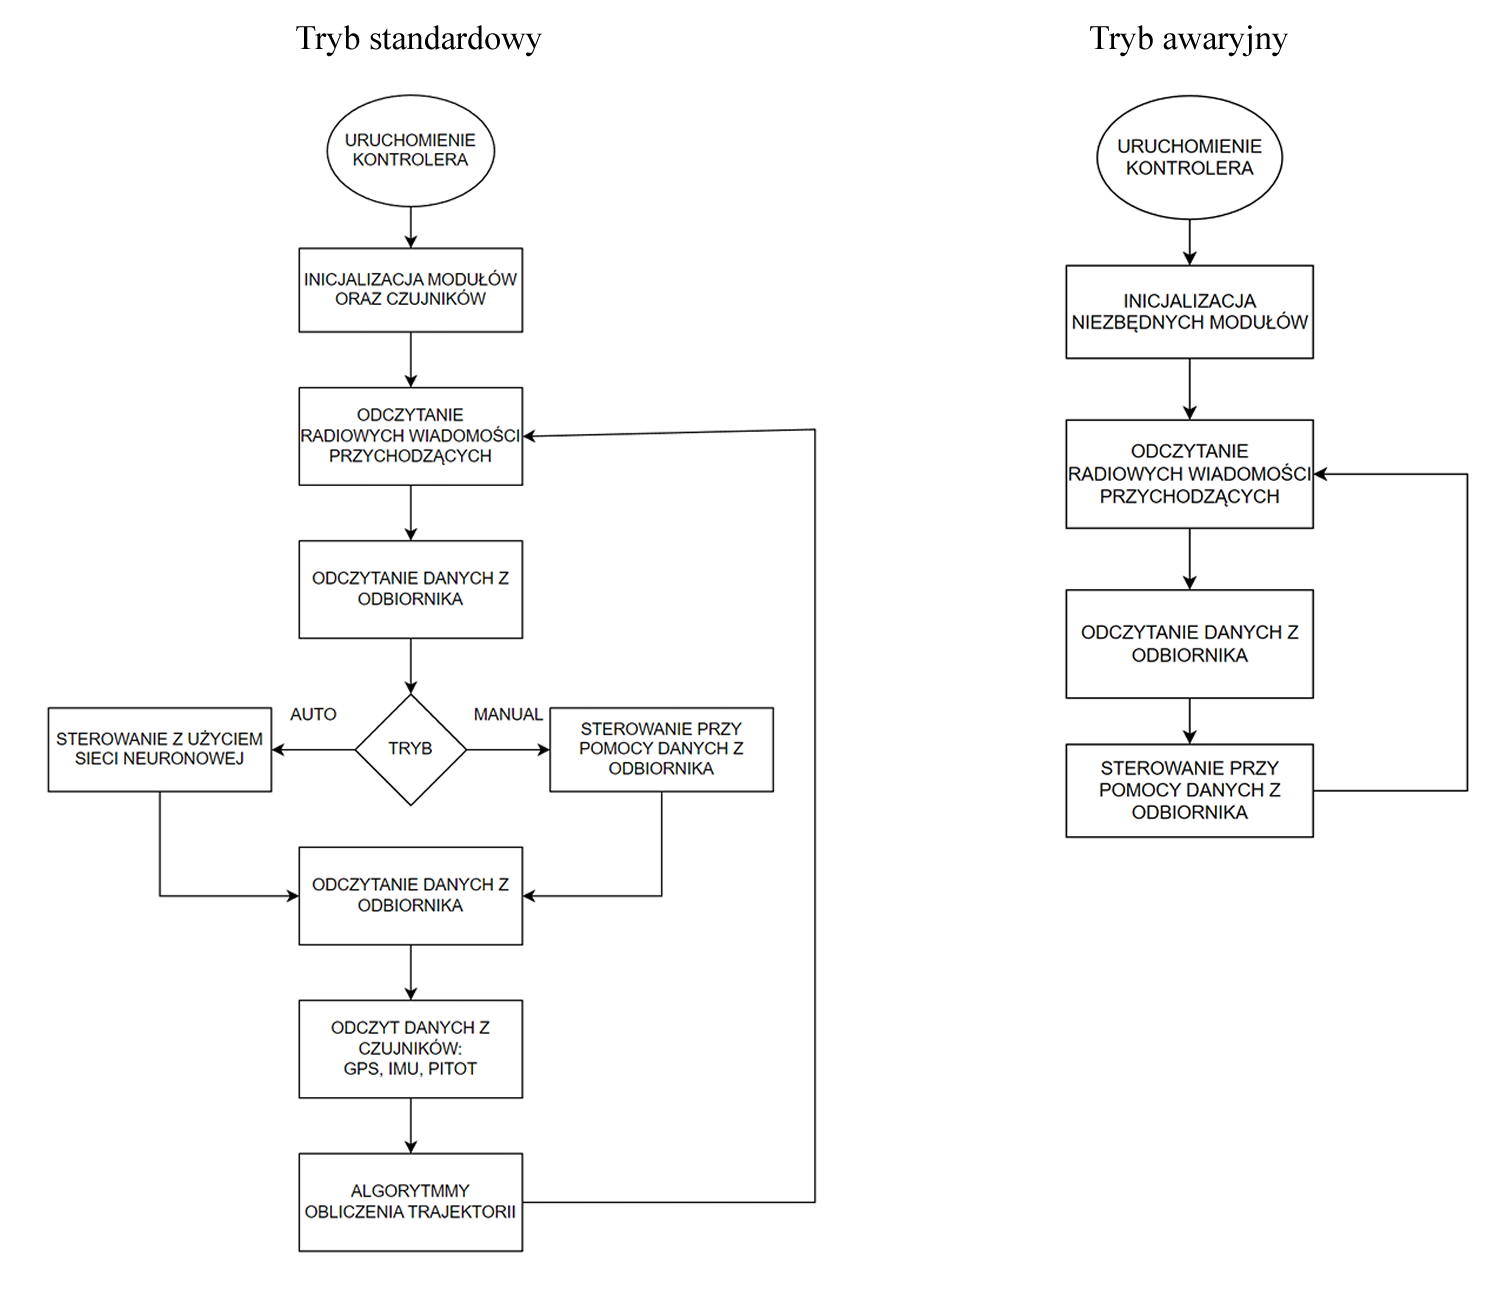
\includegraphics[width=1\textwidth]{diagramy}
    \caption{A nice plot.}
\end{figure}

Poszczególne elementy programu wykonywane są z różna częstotliwością, zależną najczęściej od szybkości działania czujnika:

\begin{center}

\begin{tabular}{| l | l |}
\hline
Element programu & Częstotliwość działania \\
\hline
Odczyt danych z odbiornika & 50 Hz \\
Sterowanie – tryb manualny & 50 Hz \\
Sterowanie – tryb autonomiczny & 20 Hz \\
Odczyt danych z sensora IMU & $\sim$100 Hz \\
Odczyt danych z rurki Pitota & 20 Hz \\
Odczyt danych z modułu GPS & 10 Hz \\
Odczyt wiadomości radiowych & $\sim$1000 Hz \\
\hline

\end{tabular}

\end{center}

Warto zauważyć, że odbiór danych z czujnika IMU odbywa się z prędkością około 100 MHz - wynika to z faktu, że algorytm DMP powinien pobrać zakolejkowane w buforze najszybciej, jak to będzie możliwe, co znacznie zwiększa precyzję działania sensora. W każdej pętli wysyłane do modułu jest zapytanie, czy nowe dane są dostępne i jeżeli tak, są one pobierane. Użyty moduł GPS jest w stanie generować nową pozycję z częstotliwością do 25 Hz, jednak przy prędkości przelotowej samolotu, pozycja generowana częściej niż 10 razy na sekundę mieści się w zakresie niedokładności pomiarowej modułu. Odczyt wiadomości radiowych odbywa się z tak wysoką częstotliwością, ponieważ odbywa się w każdej iteracji głównej pętli programu, której średni czas wykonania jest nieco niższy niż 1ms i zależy od ilości operacji wykonanych podczas niej.


Dane z rurki Pitota pełniącej funkcję czujnika prędkości wiatru względem samolotu, nie są w żaden sposób filtrowane po stronie sensora, dlatego na wyniki został nałożony algorytm średniej kroczącej kilku ostatnich wyników.

Niestety wykorzystanie zewnętrznych bibliotek do czujników, dostępnych w oficjalnych źródłach producenta, nie pozwala na pełne zarządzanie czasem pracy i oczekiwania procesora. Najbardziej newralgicznym punktem, mogącym zaburzyć działanie pracy kontrolera, jest oczekiwanie na dane przychodzące na magistrali $I^2C$ - w przypadku błędu po stronie sensora lub innego przerwania połączenia, czas ten może wynosić nawet kilkadziesiąt milisekund, co przekłada się na całkowitą utratę kontroli nad samolotem. Dlatego wprowadzone zostało dodatkowe zabezpieczenie - po wykryciu takiego błędu kontroler wchodzi w tryb awaryjny, który pozwala tylko i wyłącznie na sterowanie samolotem w trybie manualnym oraz odbieranie komend ze stacji bazowej. Wszystkie czujniki pozostają wyłączone do czasu rozbrojenia silniki i restartu urządzenia.

W pamięci EEPROM mikrokontrolera zapisywane są dane dotyczące kalibracji lokalnego  układu współrzędnych, dzięki czemu nie trzeba ich wysyłać za każdym razem po uruchomieniu systemu - są to pozycje obydwu kolumn, skala w dwóch osiach oraz kąt zawarty między równoleżnikiem a półprostą zaczynającą się w lewej kolumnie i przechodzącej przez prawą. W pamięci zapisana jest też informacja o uzbrojeniu silnika oraz lokalizacje kolejnych waypointów. Sumarycznie wykorzystane są 142 bajty pamięci. Planowane było wykorzystanie zewnętrznej pamięci EEPROM lub tej wbudowanej w mikrokontroler do aktualizowania algorytmu sieci neuronowej bez konieczności podłączania kabla, jednak takie rozwiązanie okazało się być niepraktyczne ze względu na ilość wysyłanych danych i konieczność sprawdzenia ich poprawności. Dodatkowo ponowne inicjalizowanie sieci stworzonej przy użyciu gotowych bibliotek mogło się okazać niemożliwe. Przyjętym rozwiązaniem został ulepszony dostęp do portu USB mikrokontorlera, co pozwala na aktualizację oprogramowania w zaledwie kilka sekund, a sieć zapisana jest w pamięci ROM.

\FloatBarrier
\paragraph{Algorytm estymacji trajektorii}\mbox{}

Jednym z najważniejszych aspektów wykonania precyzyjnego manewru samolotem jest wzięcie pod uwagę kilku kolejnych punktów na planowej trasie, ze względu na charakter zachowania się tego typu statku powietrznego w powietrzu. Aby umożliwić jak najkrótszy czas przygotowania samolotu do lotu, jego trasa określana jest przy pomocy pozycji dwóch kolumn, wokół których automatycznie ustalane są waypointy. Aby umożliwić dodatkową konfigurację obliczenia te prowadzone są po stronie aplikacji webowej, a następnie wysyłane na samolot. Dla ułatwienia obliczeń i wizualizacji, po skalibrowaniu terenu, samolot korzysta z lokalnego układu współrzędnych, do którego transponowane są koordynaty GPS. Powierzchnia, po której porusza się samolot jest na tyle mała w skali krzywizny Ziemii, że przyjąć można lokalny układ współrzędnych jako dwuwymiarowy układ kartezjański. 

Uwaga: zgodnie z założeniem projektowym obszar lotu oraz odległość między kolumnami są stałe. 

Aby wyznaczyć trajektorię lotu, należy najpierw określić, między którymi waypointami znajduje się samolot. Na początku działania programu zakładamy, że znajduje się przed pierwszym, a następnie sprawdzamy następujący warunek: wyznaczana jest prosta przechodząca przez kolejny punkt na trasie tak, aby kąty zawarty między nią a prostymi przechodzącymi przez kolejny punkt i sąsiadujące punkty były równe. Jeżeli pozycja samolotu wprowadzona do równania takiej prostej będzie mieć przeciwny znak, niż po wprowadzeniu pozycji poprzedniego punktu, można uznać punkt za zaliczony. 

 \begin{figure}[ht]
    \centering
    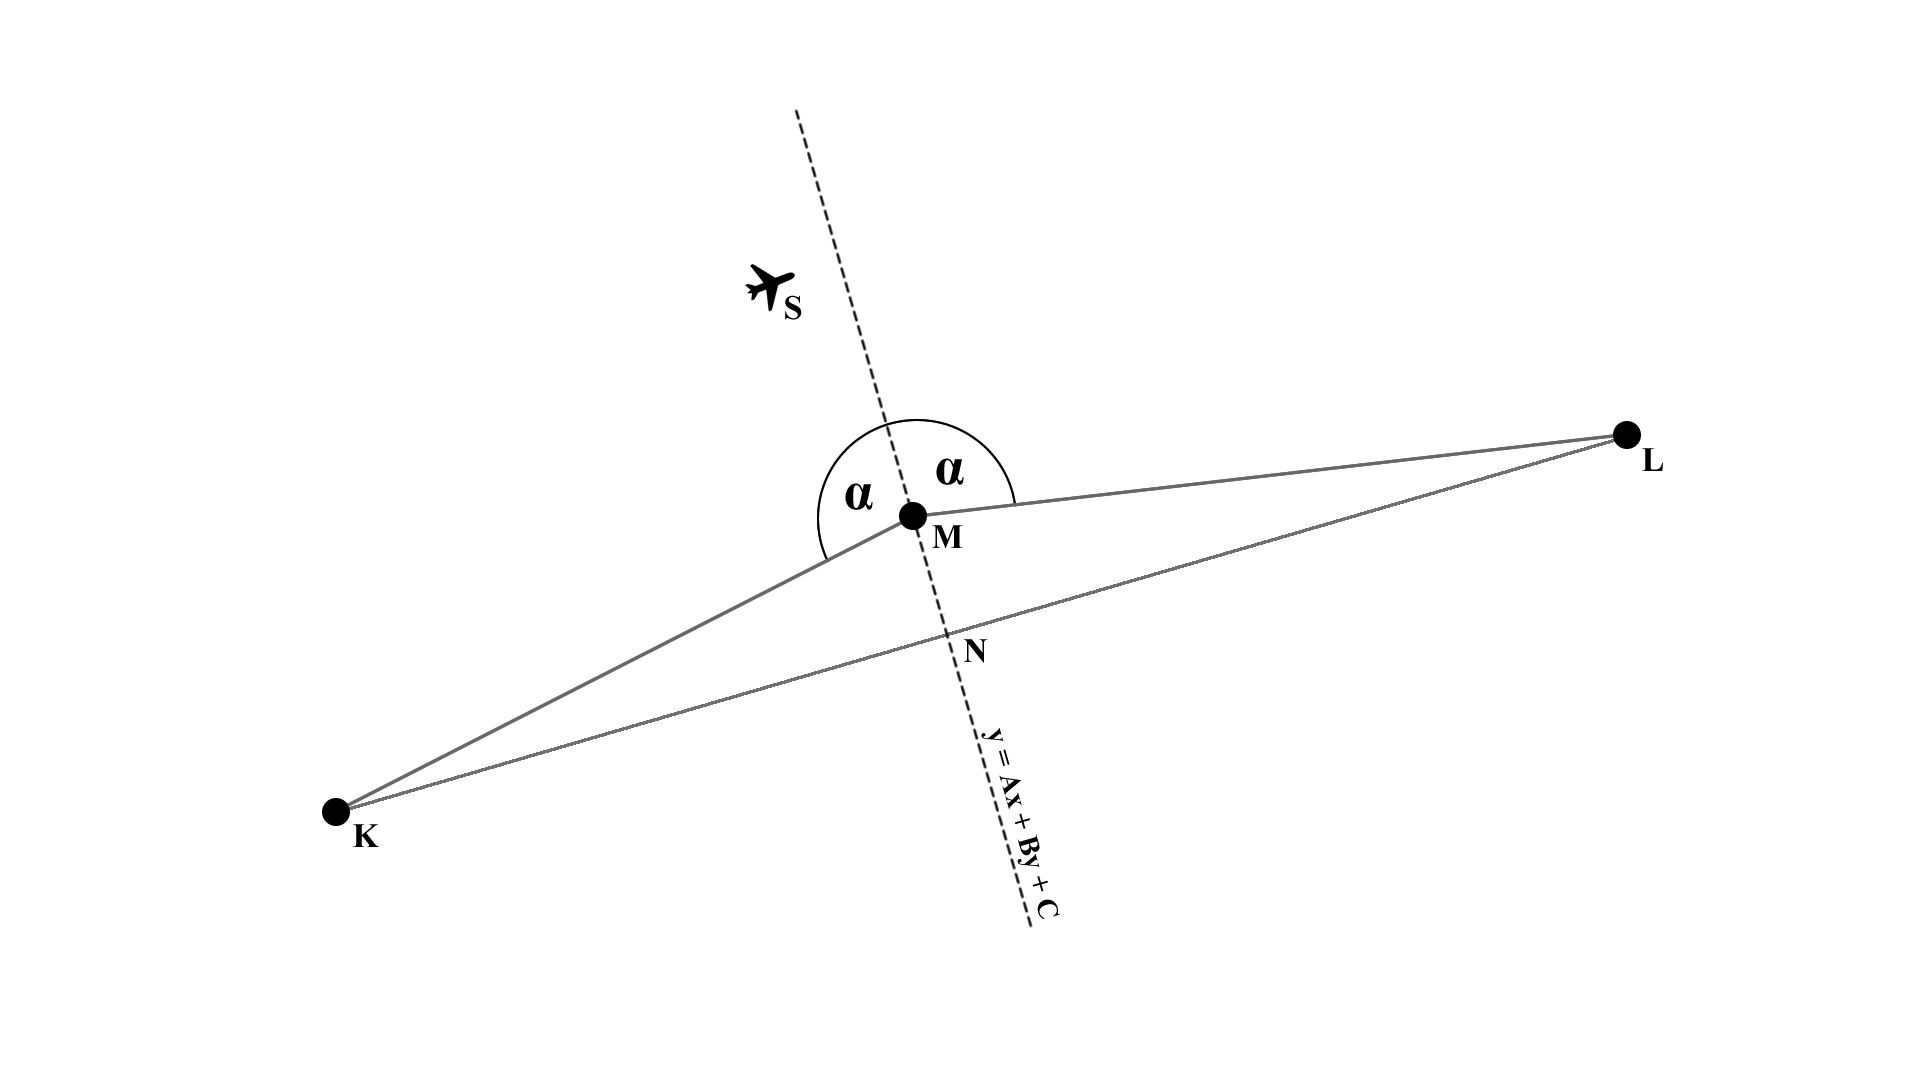
\includegraphics[width=1\textwidth]{nextwaypoint}
    \caption{Dodać podpis :)}
\end{figure}

\begin{gather*} 
	\text{Szukana prosta jest opisana równaniem:} \\ 
	y = Ax + By + C \\ 
	\text{Korzystając z twierdzenia o dwusieczej kąta w trójkącie:} \\	
	\frac{|KM|}{|LM|} = \frac{|KN|}{|LN|} \\
	=>|KN| = \frac{|KL|}{1+\frac{|KM|}{|KM|}} \\
	\vec{KN} = [L_x - K_x, L_y - K_y] \frac{|KN|}{|KL|} \\
	\text{Zatem:} \\
	A = -\frac{M_y - N_y}{M_x - N_x} \\
	B = 1 \\
	C = -N_y - A \cdot N_x \\
	y(x, y) = Ax + By + C  \\
	\text{Linia zmiany puntu zostaje przekroczona, jeśli:} \\
	H(y(S_x, S_y)) \neq  H(y(K_x, K_y)) \\
	\text{Gdzie:} \\
	H(x) = \begin{cases} 1, & x >= 0 \\ -1, & x < 0 \end{cases}	 
\end{gather*}
 \begin{figure}[ht]
    \centering
    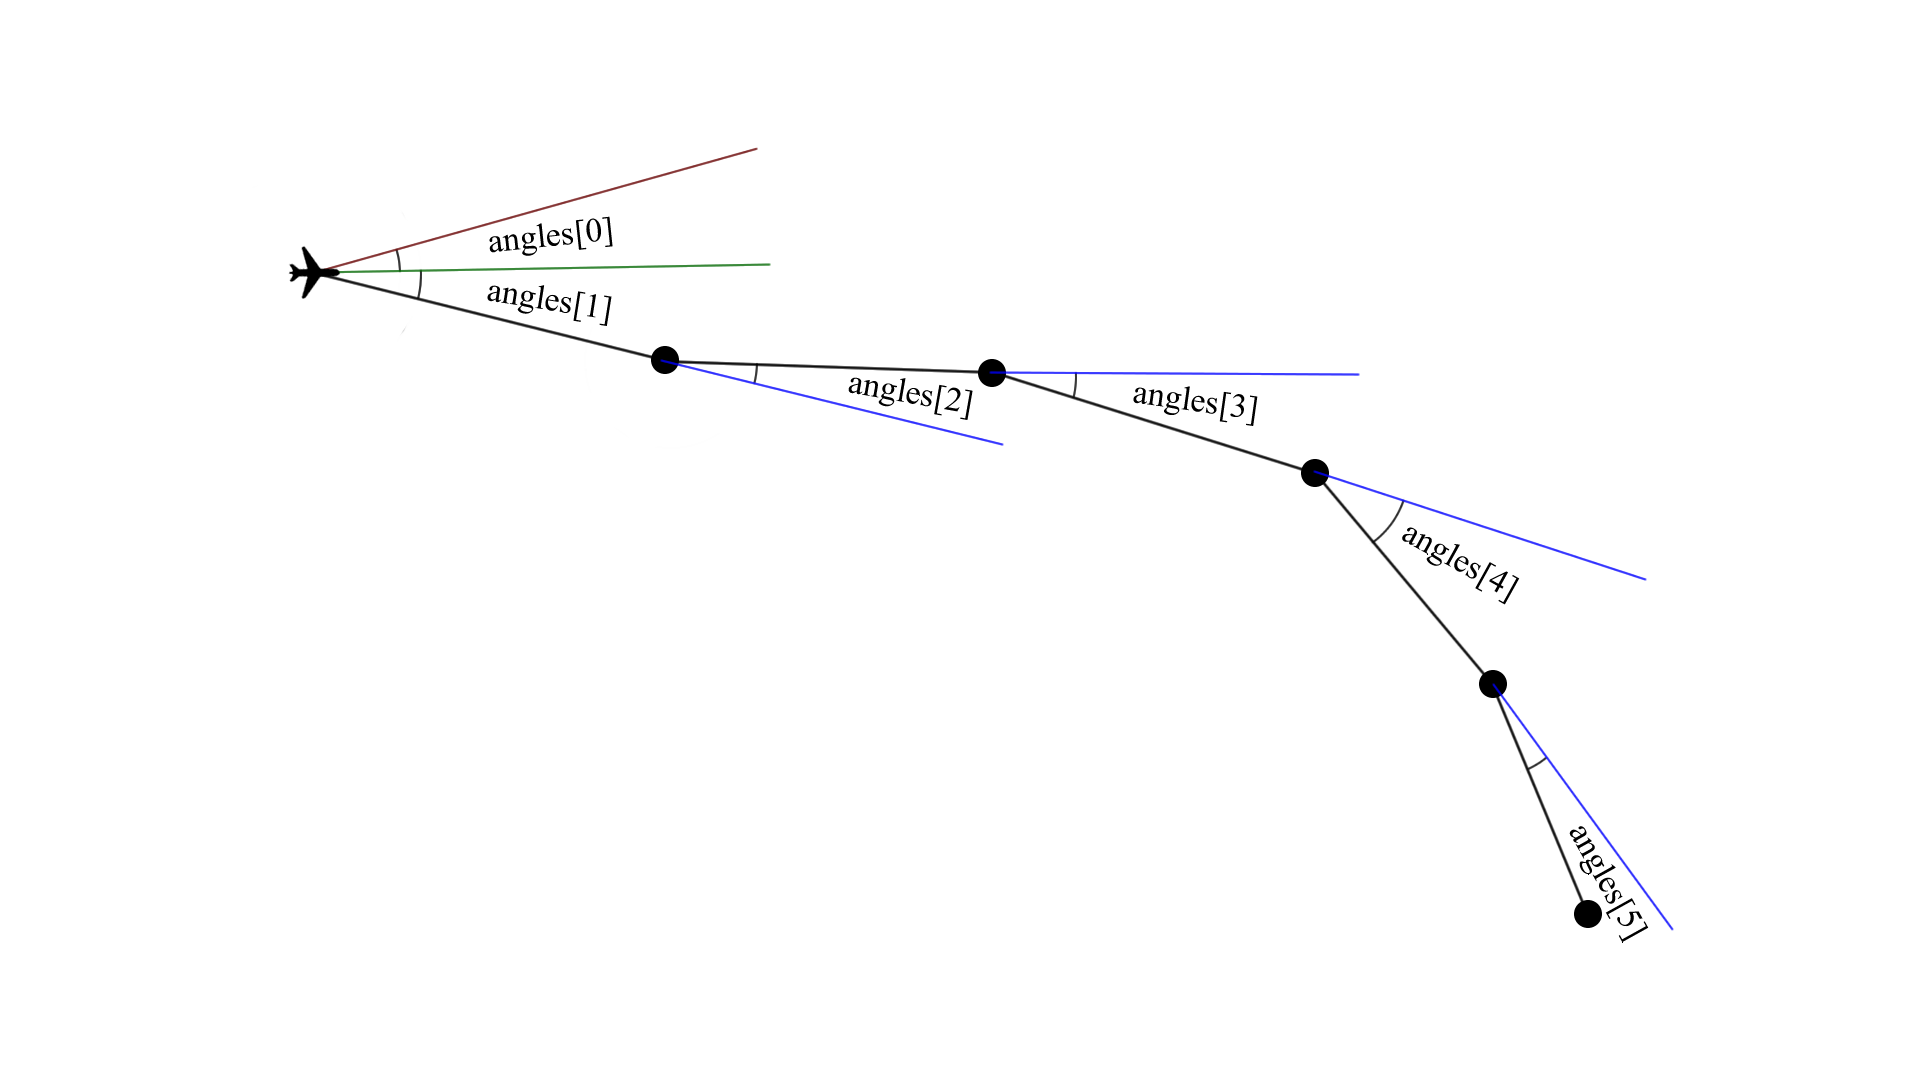
\includegraphics[width=1\textwidth]{angles}
    \caption{Dodać podpis :)}
\end{figure}
Kąty pomiędzy zawarte pomiędzy kolejnymi punktami obliczane są według poniższej zależności, zgodnie ze wzorem na kąt zawarty pomiędzy dwoma wektorami:
\begin{gather*} 
	\text{Przyjmujemy A, B, C jako kolejne punkty} \\ 
 	\vec{a} = [A_x - B_x, A_y - B_y] \\
 	\vec{b} = [C_x - B_x, C_y - B_y] \\
 	angle = 	\arccos{\frac{\vec{a} \cdot \vec{b}}{|\vec{a}||\vec{b}|} } \cdot H(a_x b_y -  a_y b_x) \\ 
 	Gdzie:
 	H(x) = \begin{cases} 1, & x >= 0 \\ -1, & x < 0 \end{cases}\\
\end{gather*}

Cała definicja trasy składa się więc z kąta zawartego między osią samolotu a trasą do najbliższego punktu i odległości do niego, kąta zawartego między osią samolotu a kierunkiem rzeczywistego poruszania się samolotu oraz kątów zawartych między pozycjami samolotu i następujących po sobie punktach na trasie. Odległości między waypointami są zbliżonymi do siebie wartościami, można przyjąć je jako równe. Sumarycznie otrzymujemy dziewięć wartości, co pozwala przewidzieć trasę na około 60 metrów czyli kilka sekund lotu. Warto zauważyć, że trzy pierwsze kąty oraz odległość do najbliższego punktu zmieniają się w czasie rzeczywistym wraz z ruchem i rotacją samolotu, pozostałe wartości zmieniają się po przekroczeniu linii zmiany waypointa. 

Uwaga: zgodnie z założeniem projektowym, wszystkie punkty znajdują się na tej samej wysokości. Z perspektywy programu możliwe by było wprowadzenie trzeciej zmiennej pozycji, jednak trening podczas lotu manualnego, w trakcie którego zbierane są dane testowe, oszacowanie wysokości, na której znajduje się samolot jest bardzo nieprecyzyjne, i mogło by negatywnie wpłynąć na wynik działania kontrolera.



 \FloatBarrier
\subsection{Stacja odbiorcza}
Wszystkie dane wysyłane przez moduł radiowy z pokładu samolotu są odbierane przez ten sam układ HC-12 znajdujący się w naziemnej stacji odbiorczej, w skład której wchodzi jeszcze mikrokontroler Arduino Mega. Posiada on kilka wbudowanych portów UART, dlatego idealnie nadaje się jako przekaźnik sygnału do portu USB na komputerze.
 \begin{figure}[ht]
    \centering
    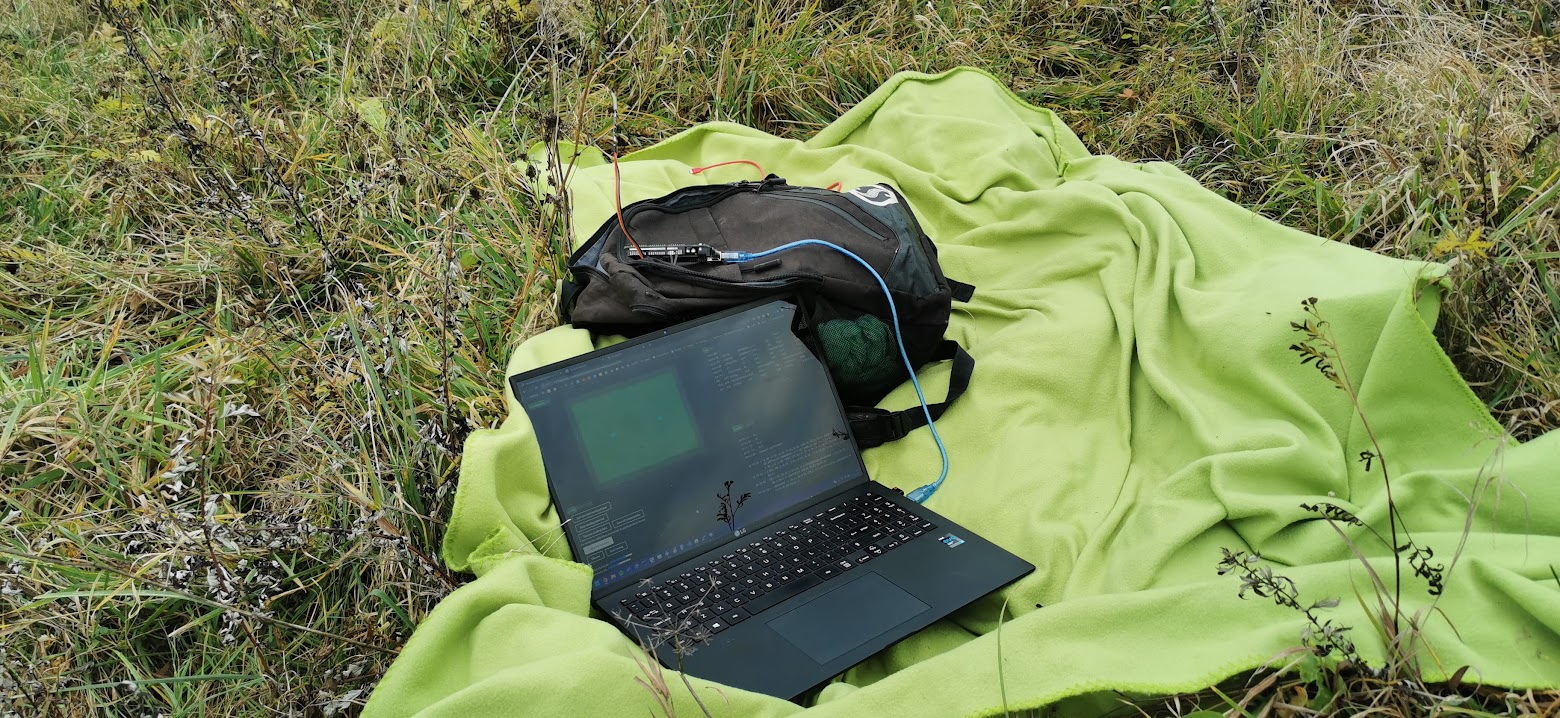
\includegraphics[width=1\textwidth]{stacjaodbiorcza}
    \caption{Dodać podpis :)}
\end{figure}

Programem obsługującym dwustronną komunikację ze stacją odbiorczą jest przygotowany w języku Python3 skrypt, który nasłuchuje zarówno wiadomości od serwera oraz z Arduino i przekazuje je dalej, w odpowiednim kierunku. Wspomniany serwer jest natomiast aplikacją stworzoną w środowisku NodeJS, w języku JavaScript. Działa on jako serwer komunikacji w protokole WebSocket, umożliwiającym praktycznie natychmiastową komunikację pomiędzy podłączonymi wcześniej klientami. Jego zadaniem jest zdekodowanie odbieranych danych i przekazanie do miejsc docelowych. Dzięki temu, webowa aplikacja może być na raz uruchomiona na kilku komputerach. Magazynuje także dane zbierane podczas lotu w formie plików dostępnych do pobrania. Serwer ten mógłby zostać uruchomiony w sieci lokalnej (na przykład na laptopie, do którego podłączona jest stacja odbiorcza), jednak w praktyce wygodniejsze okazało się zainstalowanie jej na domowym serwerze, do którego dostęp jest przez sieć Internet.
 \begin{figure}[ht]
    \centering
    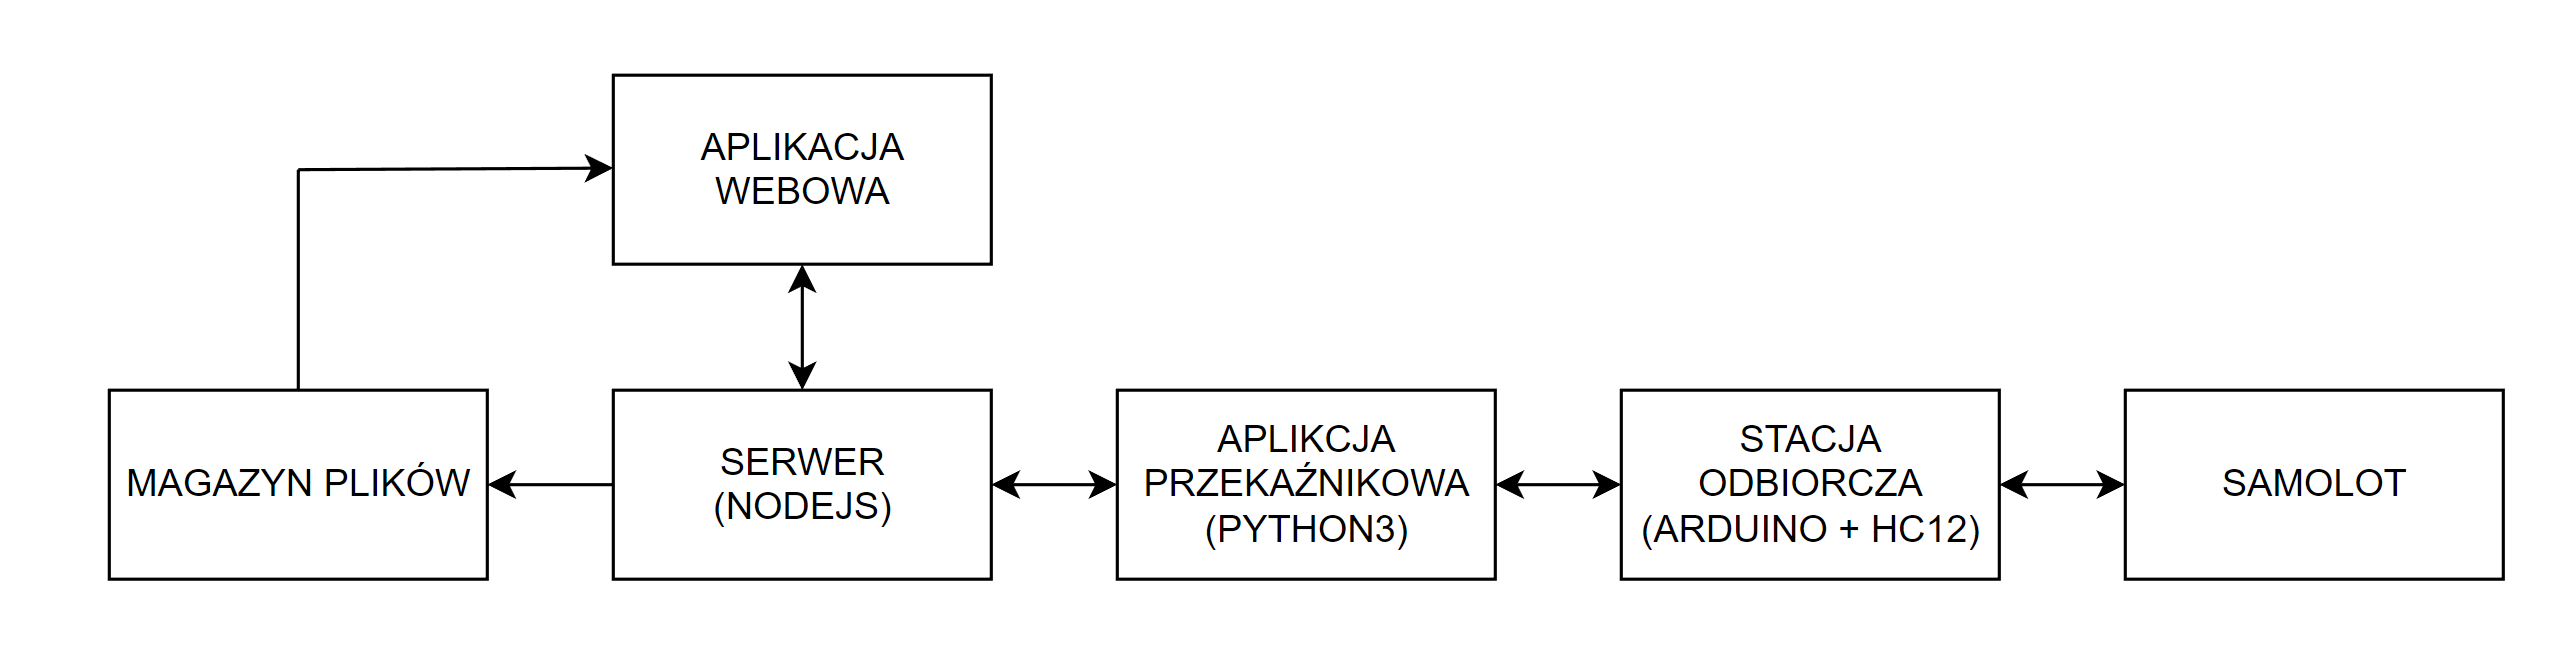
\includegraphics[width=1\textwidth]{diagram_env}
    \caption{Dodać podpis :)}
\end{figure}

Warto wspomnieć, że komunikacja odbywa się przez moduły HC-12, które są tansceiverami (połączeniem transmittera oraz receivera), czyli umożliwia komunikację dwustronną. Moduł ten ma pewne ograniczenia, widoczne przede wszystkim przy próbie równoczesnego nadawania oraz odbierania danych. Po uruchomieniu transmisji, samolot nadaje dane w trybie praktycznie ciągłym, dlatego wysłanie do niego ramki danych jest bardzo utrudnione i mało prawdopodobne. Dlatego na aparaturze jeden z przełączników działa jako blokada transmisji danych (od strony oprogramowania kontrolera), która umożliwia na bezproblemową komunikację.

\FloatBarrier
\subsection{Protokół komunikacji}
Komunikacja między poszczególnymi elementami systemu wymagała opracowania dedykowanego protokołu komunikacyjnego tak, aby każda wiadomość trafiła w odpowiednie miejsce i została prawidłowo odczytana. 
Komunikacja pomiędzy stroną internetową, serwerem i aplikacją przekaźnikową odbywa się przy pomocy ramek w notacji JSON. Wiadomość zawiera pole type, oznaczające rodzaj wiadomości - na tej podstawie poszczególne programy wiedzą w jaki sposób odczytać resztę wiadomości. Poszczególne ramki zawierają dodatkowe pola z informacjami. 

Komunikacja między samolotem a stacją naziemną jest narażona na zakłócenia spowodowane odległością oraz brakiem dodatkowego kodowania wiadomości. Dlatego wiadomości muszą być maksymalnie krótkie a algorytm je odczytujący odporny na otrzymanie niekompletnej ramki. Przygotowane zostały trzy typy wiadomości:
1.	Zapytanie o wartość - składające się ze znaku ? oraz docelowej zmiennej
2.	Nakaz zmiany wartości - składa się ze znaku !, docelowej zmiennej oraz nowej wartości w postaci liczby zmiennoprzecinkowej
3.	Nakaz wykonania akcji - składające się ze znaku @ oraz numeru akcji.
Każda liczba musi być zakończona znakiem ;. Poszczególne znaki (w tym także kolejne cyfry) są kodowane w postaci znaków ASCII, co zmniejsza ryzyko wystąpienia błędu odczytu informacji - ramka prędzej zostanie utracona niż błędnie zinterpretowana. W odpowiedzi na zapytania o wartości lub przy różnych akcjach samolot może wysłać ramkę zwrotną w postaci: \#, kod informacji, wartość. Kodowane w ten sposób wiadomości są istotne z punktu widzenia pozostałych programów w środowisku. Wiadomości informacyjne lub debugujące mogą zostać wysłane w postaci zwykłego tekstu, który zostanie wyświetlony na konsoli w aplikacji internetowej. 

Przykładowa ramka: 

?3;  - odeślij lokalizację lewej kolumny
!0;1; - zmień tryb wysyłania danych na ciągły
@0; - uzbrój samolot

Przykładowa odpowiedź:
\#5;1; - potwierdzenie prawidłowej inicjalizacji modułu GNSS
\FloatBarrier
\subsection{Oprogramowanie naziemne}
Podczas testów samolotu bardzo szybko okazało się, że do efektywnej pracy nad modułem kontrolera konieczne będzie przygotowanie środowiska, które pozwoli na podgląd i wizualizację danych oraz konfigurację parametrów systemu. Początkowy projekt założył prosty program do wyświetlania zapisanych w pliku danych zebranych podczas przelotu w postaci wykresów.

 \begin{figure}[ht]
    \centering
    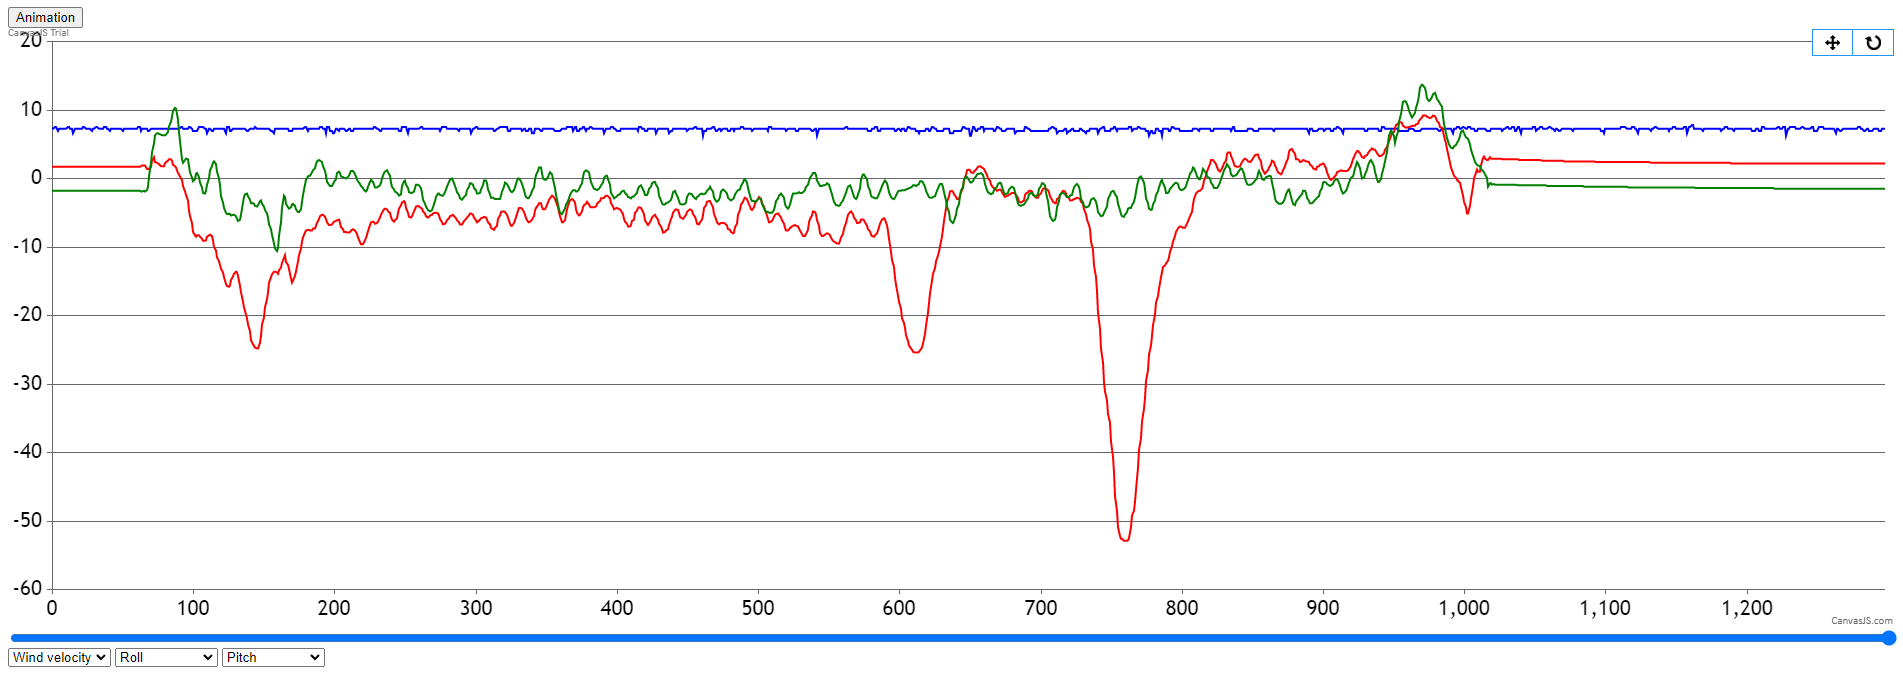
\includegraphics[width=1\textwidth]{starysystem}
    \caption{Dodać podpis :)}
\end{figure}

Program został przygotowany w formie strony internetowej tak, aby możliwy był do niego dostęp z poziomu przeglądarki. Niestety, szybko okazało się, że jest to rozwiązanie tylko tymczasowe - brak możliwości podglądu danych w czasie rzeczywistym znacząco utrudniał pracę nad samym kontrolerem - największym problemem był brak możliwości sprawdzenia poprawności działania algorytmów przetwarzające dane lokalizacyjne i estymacji trajektorii lotu. Podczas testów w warunkach polowych bardzo uciążliwa była konieczność ponownej kompilacji całego programu i ponownego wgrywania do mikrokontrolera przy każdej zmianie parametrów. 

Pojawił się więc pomysł stworzenia aplikacji, która pozwoli na podgląd danych w czasie rzeczywistym, konfigurację samolotu a także zapis i analizę zebranych danych. Projektując system największy nacisk położony został na jego przejrzystość, łatwość obsługi i praktyczność, tak aby pozwolić zaoszczędzić każdą cenną sekundę podczas wykonywania lotów testowych. 

 \begin{figure}[ht]
    \centering
    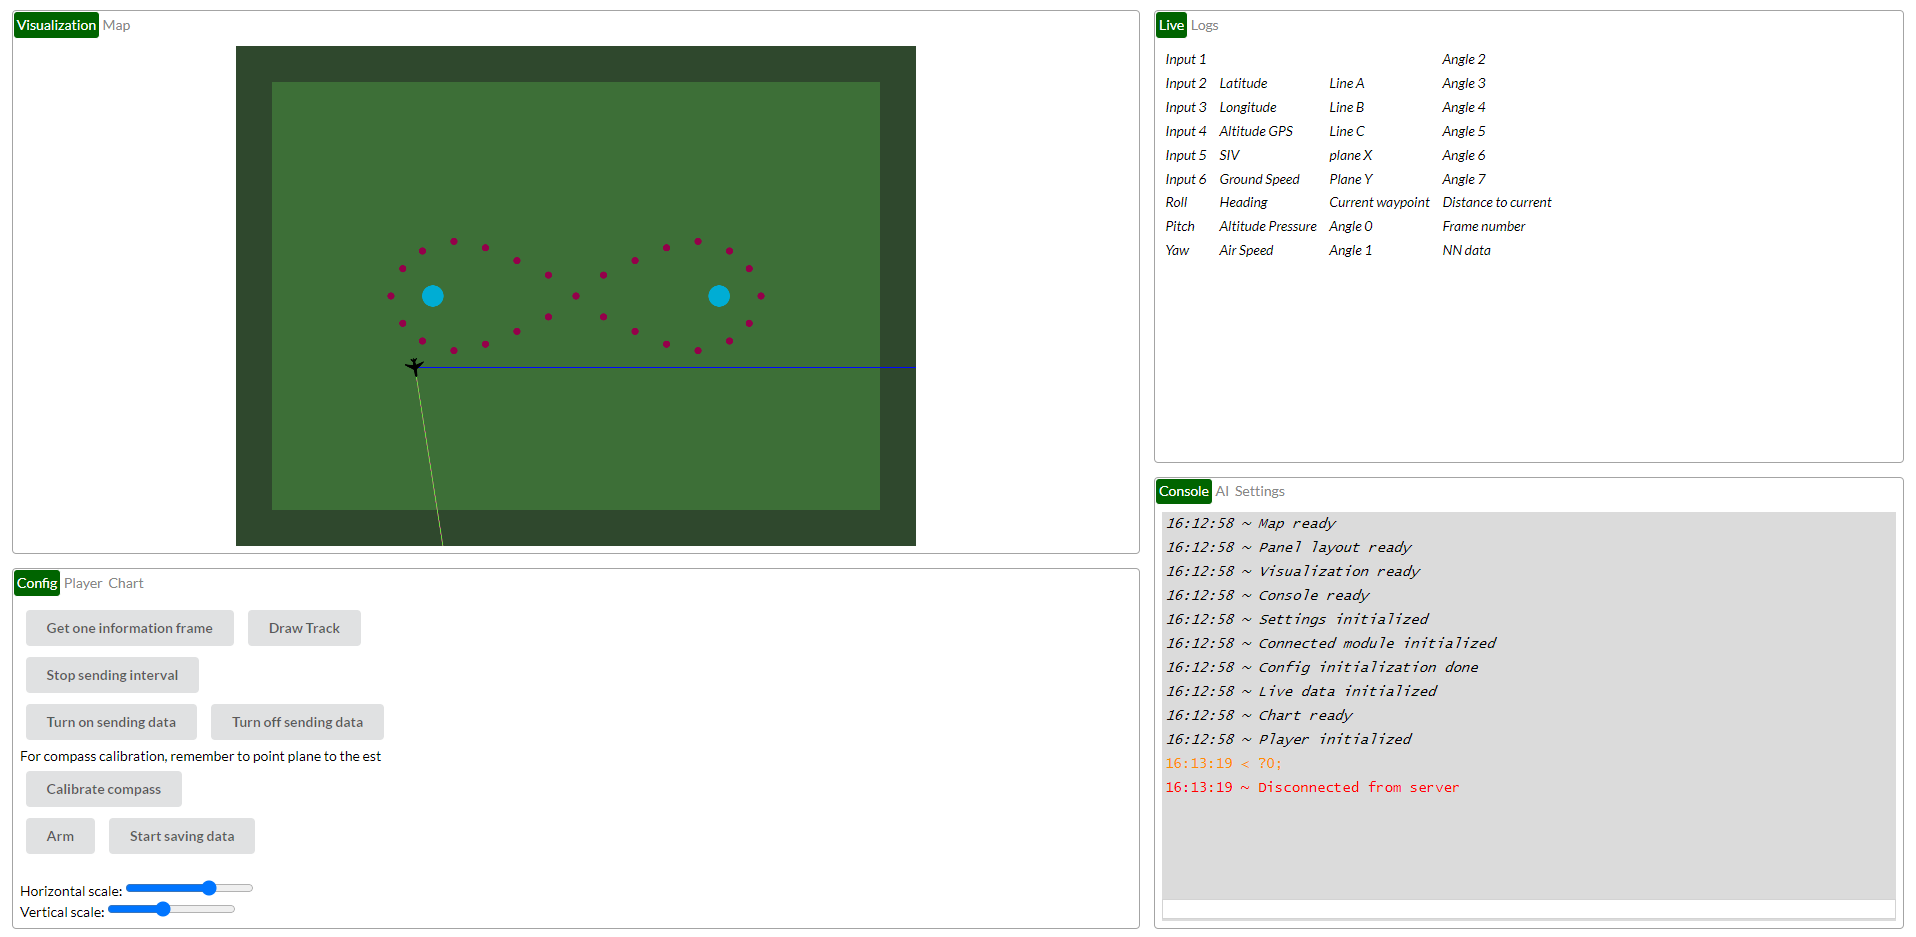
\includegraphics[width=1\textwidth]{weball}
    \caption{Dodać podpis :)}
\end{figure}



\paragraph{Układ czteropanelowy}\mbox{}

Wygląd i układ programu są najistotniejszymi elementami decydującymi o jego przejrzystości. Pierwszym pytaniem podczas projektowania tego typu oprogramowania jest zmaksymalizowanie ilości informacji, które użytkownik może równocześnie obserwować. Zgodnie z założeniem, program  miał umożliwiać pracę nad różnymi aspektami samolotu: analizę danych (w czasie rzeczywistym lub odtworzonych z pliku), konfigurację trasy czy podgląd stanu połączenia całego środowiska. Podsumowując, jedno statyczne ułożenie elementów interfejsu byłoby niemożliwe, stąd koncepcja rozwoju dynamicznego układu czteropanelowego, która pozwala na wyświetlanie różnych stron aplikacji w oknach.

Co najważniejsze, rozmiar paneli nie jest stały, można go dynamicznie modyfikować w intuicyjny sposób przy pomocy przeciągnięcia wskaźnikiem myszy. Ponadto, strony nie są przypisane do jednego panelu, można zmieniać ich lokalizację po przeciągnięciu paska tytułowego na inny obszar. Zmiana kolejności wyświetlanych stron w obrębie panelu także jest możliwa w analogiczny sposób. Całość umożliwia (w zależności od potrzeby) wyświetlanie na ekranie zupełnie innych zestawów informacji. Przełączenie się między dowolną konfiguracją zajmuje czas liczony w sekundach. Podczas kalibracji przed startem wygodniejszy będzie podgląd na mapę, sieć połączeń środowiska, ekran konfiguracji i konsolę, w trakcie lotu niezbędny jest ekran podglądu danych i wizualizacja, a podczas analizy zebranych danych panel odtwarzania czy lista plików.



System został stworzony w formie strony internetowej przy pomocy technologii: HTML, JavaScript, jQuery, jQuery-UI, Semantic-UI oraz CSS i przygotowywany głównie pod przeglądarkę Google Chrome. Dostęp do niego nie wymaga żadnej instalacji i jest możliwy za pośrednictwem internetu. 


 \begin{figure}[ht]
    \centering
    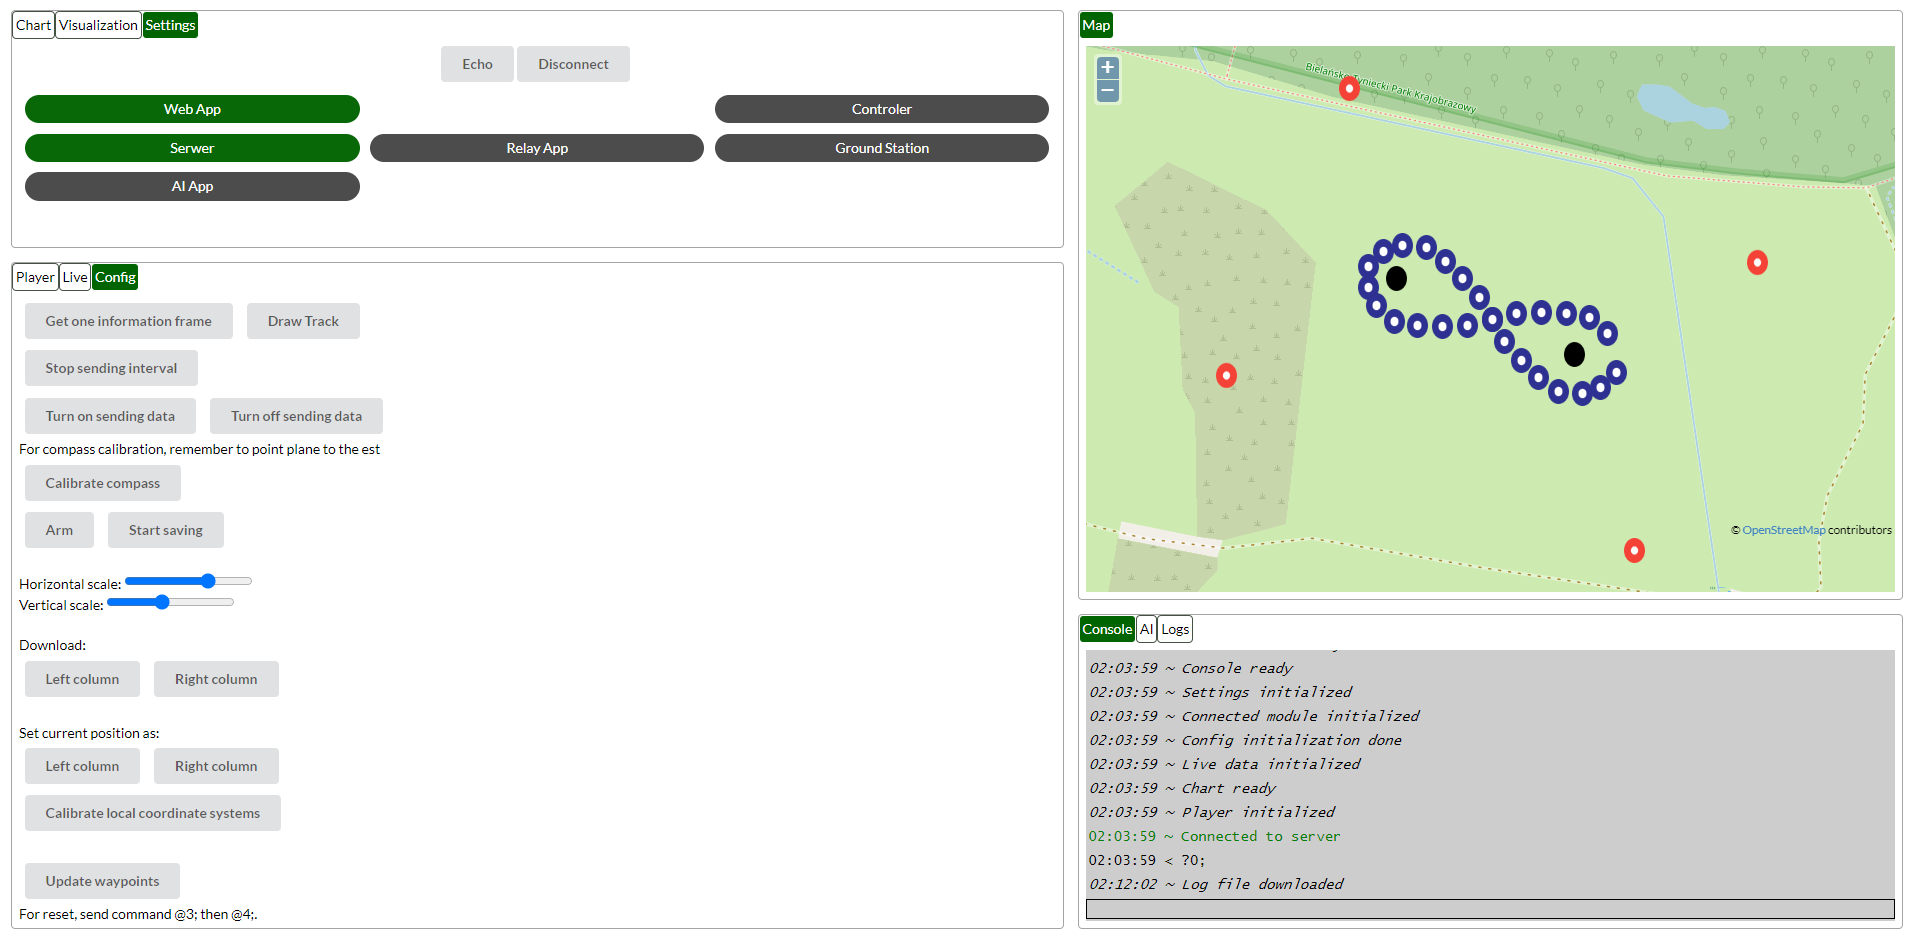
\includegraphics[width=1\textwidth]{przedlotem}
    \caption{Dodać podpis :)}
\end{figure}

 \begin{figure}[ht]
    \centering
    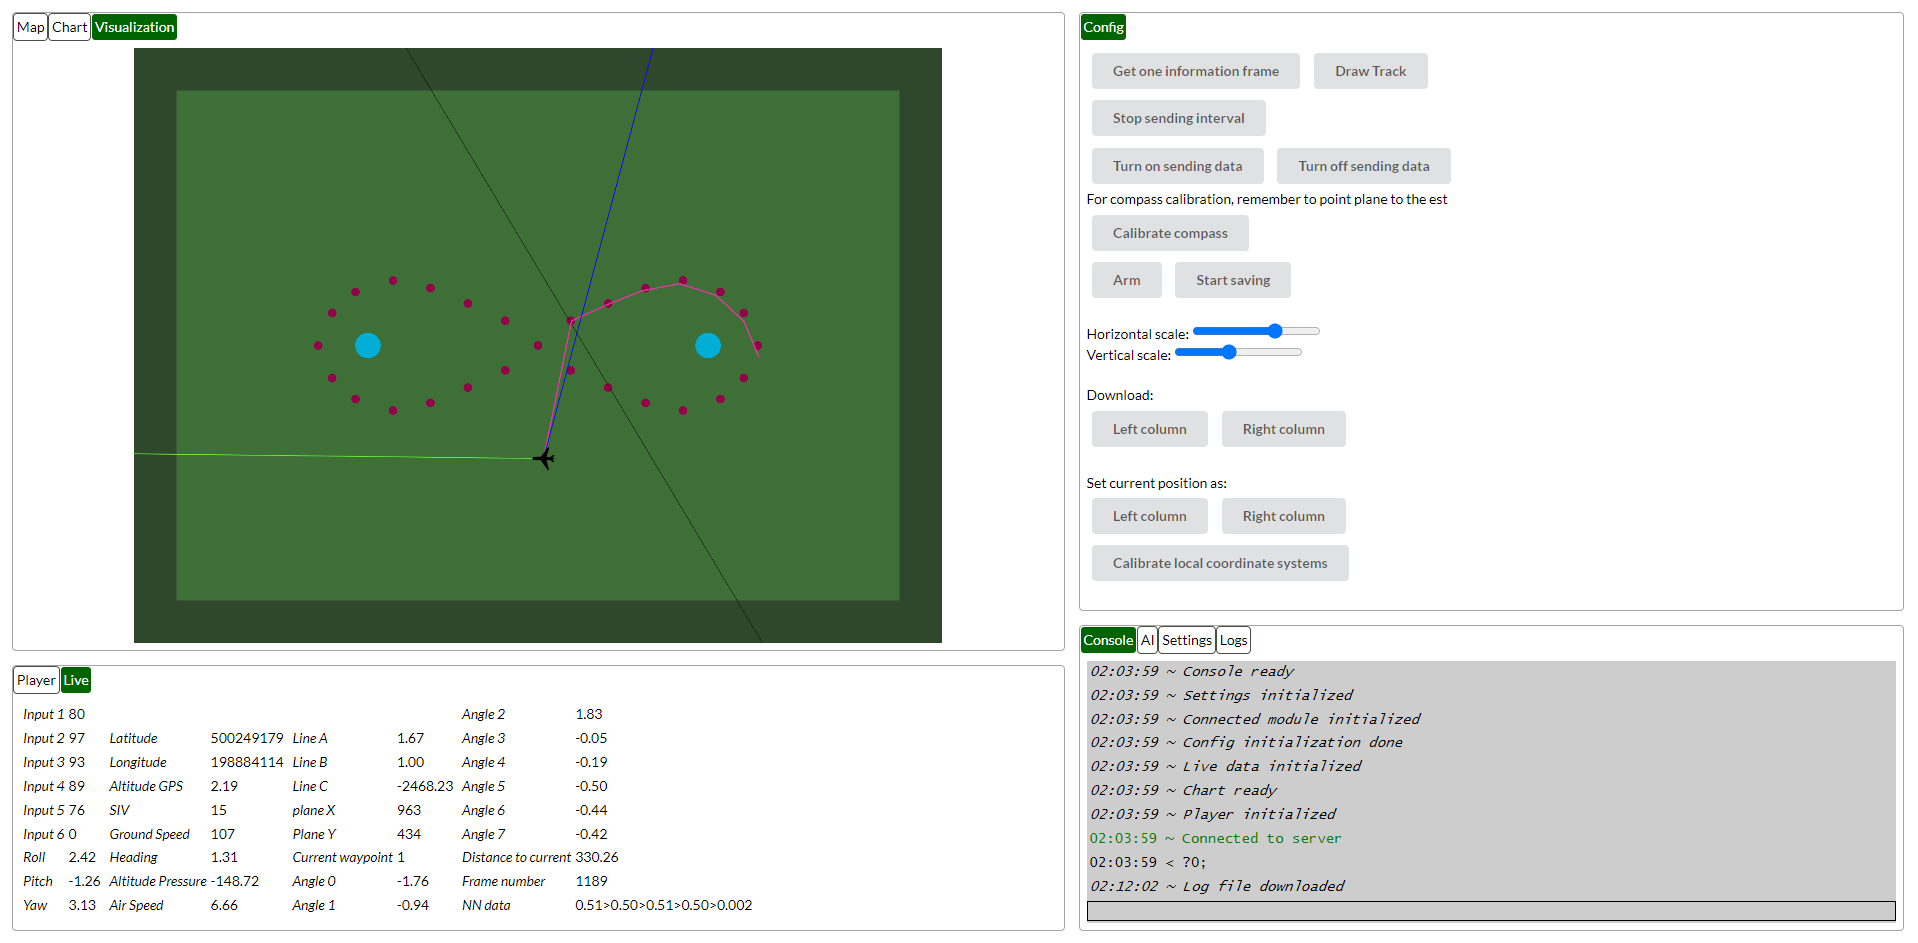
\includegraphics[width=1\textwidth]{podczaslotu}
    \caption{Dodać podpis :)}
\end{figure}

 \begin{figure}[ht]
    \centering
    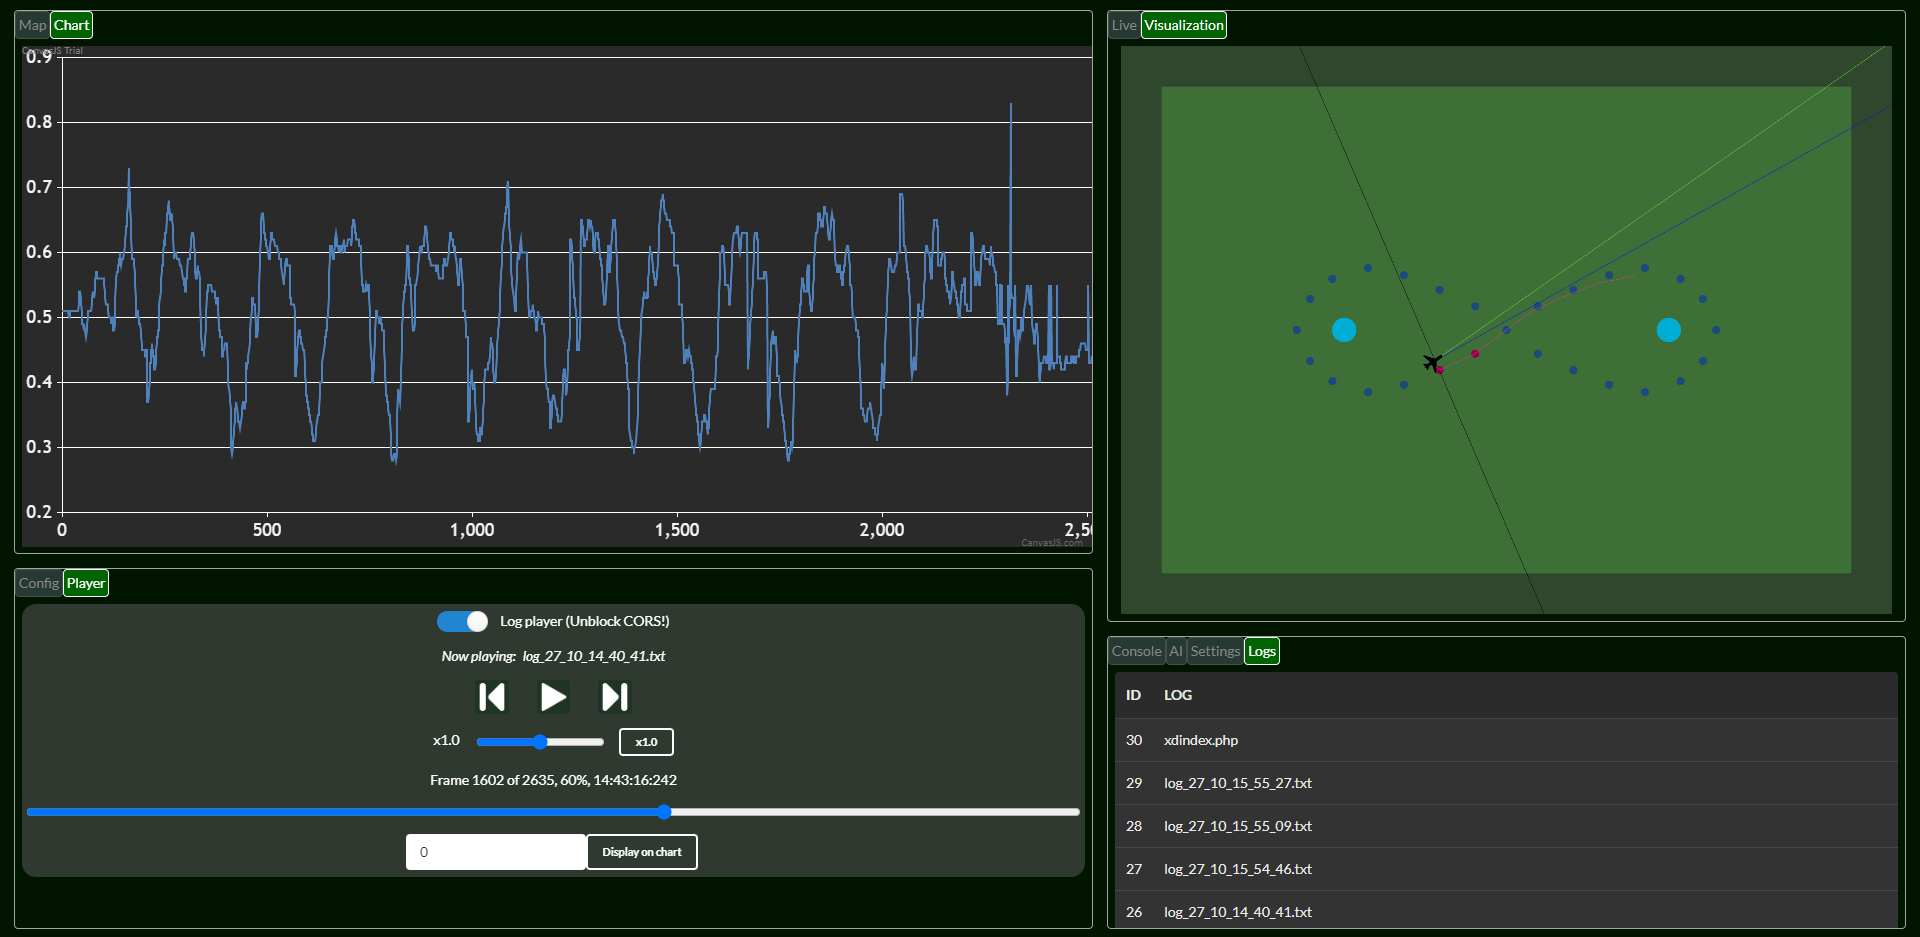
\includegraphics[width=1\textwidth]{polocie}
    \caption{Dodać podpis :)}
\end{figure}

\FloatBarrier
 
\paragraph{Strona: Wizualizacja}\mbox{}

Strona wizualizacji jest jedną z najistotniejszych zakładek pozwalających sprawdzić obecne położenie samolotu, wyznaczoną trasę oraz które z nich zostały już zaliczone. Podczas tworzenia algorytmów transformacji do lokalnego układu współrzędnych oraz estymacji trajektorii podgląd taki okazał się niezbędny, zwłaszcza na etapie weryfikacji poprawności ich działania - dane liczbowe często mogły się wydawać poprawne, jednak dopiero ich wizualizowanie pozwoliło na bardzo dokładne sprawdzenie i wychwycenie błędów (na przykład niepoprawne skalowanie względem osi). W trakcie lotu testowego podgląd pozycji jest także wygodny jako wsparcie pilota, który nie zawsze jest w stanie poprawie określić odległość samolotu od siebie. Ponadto, możliwe jest sprawdzenie w czasie rzeczywistym kalibracji i poprawności danych. Do przygotowania modułu wizualizacji konieczna jest kalibracja lokalnego układu współrzędnych z samolotem. Bezpośrednio powiązaną stroną jest moduł wyświetlania danych w czasie rzeczywistym, które są aktualizowane na podstawie ramek przychodzących z samolotu.

 \begin{figure}[H]
    \centering
    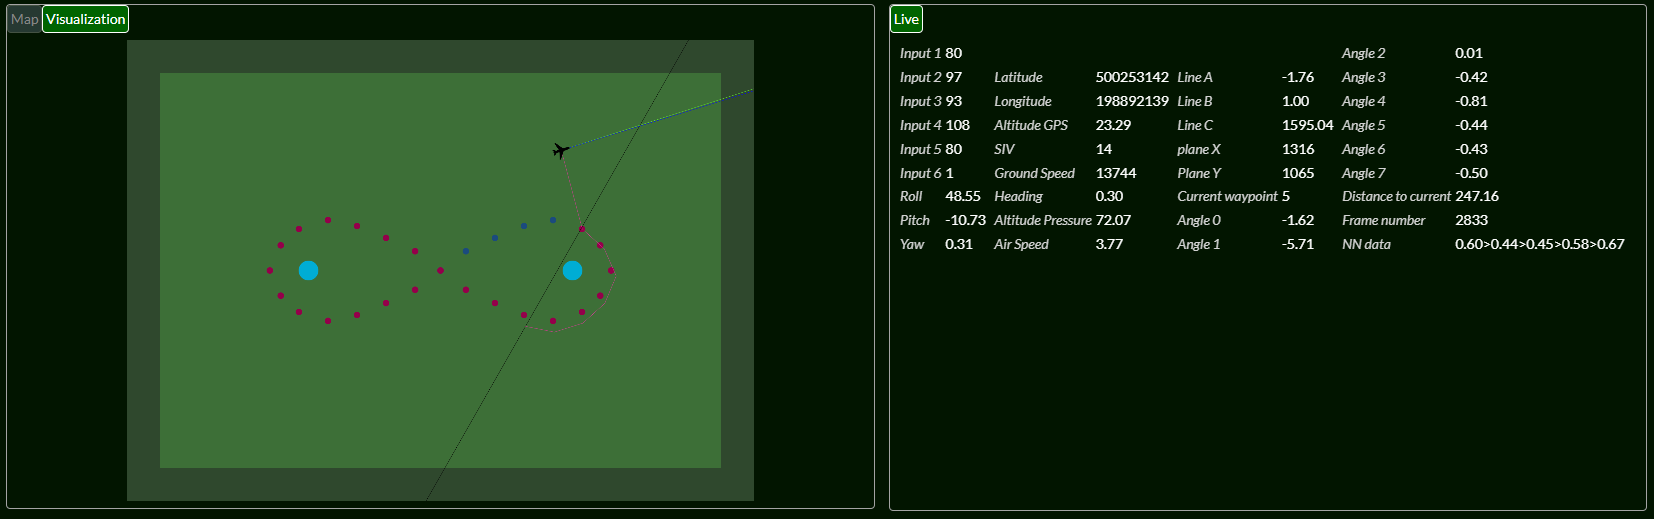
\includegraphics[width=1\textwidth]{wizualizacja}
    \caption{Dodać podpis :)}
\end{figure}

\paragraph{Strona: Mapa}\mbox{}

Podczas przygotowań do lotu i przy wyznaczeniu obszaru lotu oraz jego trasy, pomocne może być określenie położenia samolotu na mapie terenu. W tym celu wykorzystano działające na licencji open source Open Street Maps poprzez bibliotekę OpenLayers. Na mapie naniesiona jest lokalizacja samolotu a także słupy, trasa oraz obszar lotu.

 \begin{figure}[H]
    \centering
    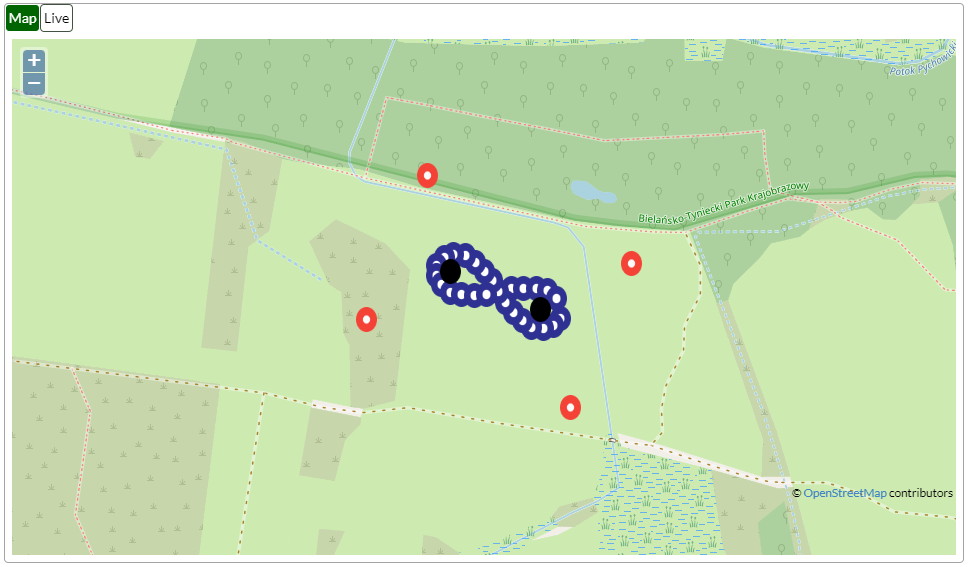
\includegraphics[width=1\textwidth]{mapa}
    \caption{Dodać podpis :)}
\end{figure}


\paragraph{Strona: Konsola}\mbox{}

Konsola została przygotowana z myślą o bezpośredniej dwustronnej komunikacji z kontrolerem, a także wyświetlania komunikatów z samolotu jak i z programu. Tekst wpisany w okno konsoli zostaje wysłany bezpośrednio do kontrolera. Interakcja z konsolą odbywa się w sposób analogiczny jak w najczęściej używanych tego typu aplikacjach - pozwala na korzystanie ze strzałek do przewijania po poprzednio wysłanych komendach, automatycznie przewija do nowych wiadomości po ręcznym przewinięciu na sam dół, a okno wpisywania staje się aktywne po kliknięciu gdziekolwiek na obszarze panelu. Dodatkowo wyświetlany tekst może być odpowiednio stylizowany oraz pokazywane jest jego źródło poprzez odpowiedni symbol przed wiadomością. Konsola przechowuje do 1000 wierszy informacji.

 \begin{figure}[H]
    \centering
    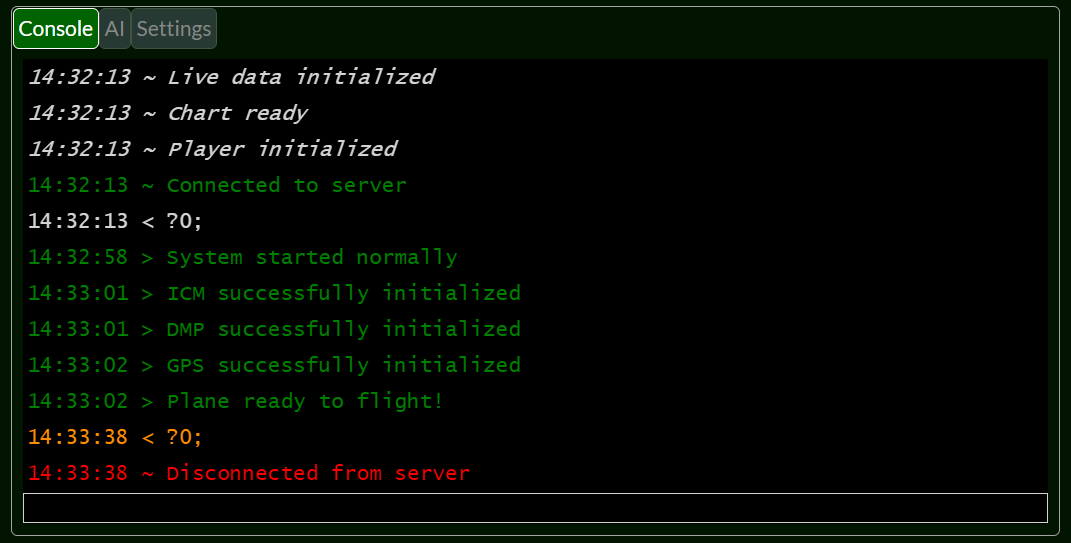
\includegraphics[width=1\textwidth]{konsola}
    \caption{Dodać podpis :)}
\end{figure}

\paragraph{Strona: Konfiguracja}\mbox{}

Strona ta jest kluczowa przy konfiguracji samolotu przed startem. Umożliwia zarządzenie wysyłaniem danych, zbrojeniem silnika, zapisem danych, kalibracją terenu czy zarządzaniem trasą. Dzięki użyciu protokołu komunikacyjnego możliwe jest automatyczne wysłanie danych, wraz z informacją zwrotną - przykładowo informacja o poprawnym odebraniu pozycji waypointa skutkuje uruchomieniu procedury wysłania kolejnego. W skład takiej procedury wchodzi wysłanie osobo obydwu współrzędnych.

 \begin{figure}[H]
    \centering
    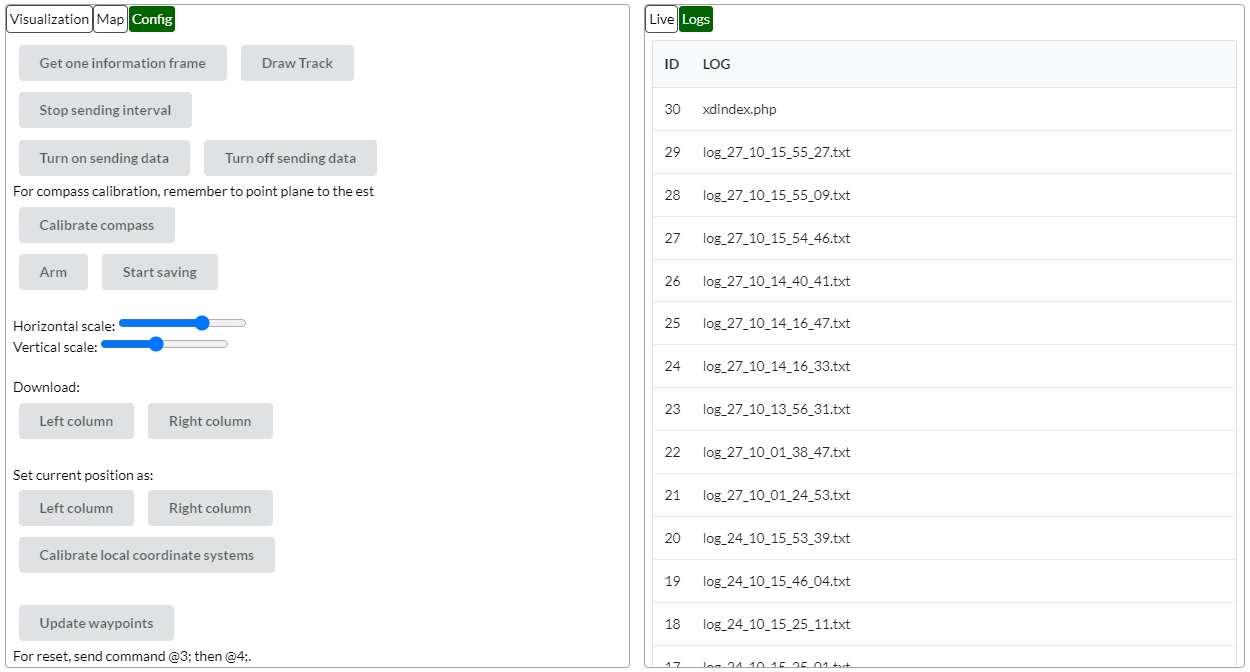
\includegraphics[width=1\textwidth]{config}
    \caption{Dodać podpis :)}
\end{figure}

\paragraph{Strona: Ustawienia}\mbox{}

Jeżeli występuje problem z podłączeniem do samolotu najszybszym sposobem do zlokalizowania newralgicznego miejsca jest zakładka Settings - za pomocą mapy połączeń w całym środowisku możliwe jest określenie błędu. Przykładowo, problem z siecią czasem może skutkować błędem aplikacji przekaźnikowej, z kolei serwer czasem automatycznie kończy działanie ze względu na brak aktywności.  Wywołanie funkcji Echo skutkuje wysłaniem prośby do kolejnych programów o odesłanie informacji o prawidłowym działaniu. Podczas pracy strona okazała się bardzo praktyczna i pozwoliła każdorazowo na oszczędzenie nawet kilku minut. Uwaga: z przyczyn praktycznych aplikacja do treningu sztucznej inteligencji nie została finalnie podłączona do środowiska.

 \begin{figure}[H]
    \centering
    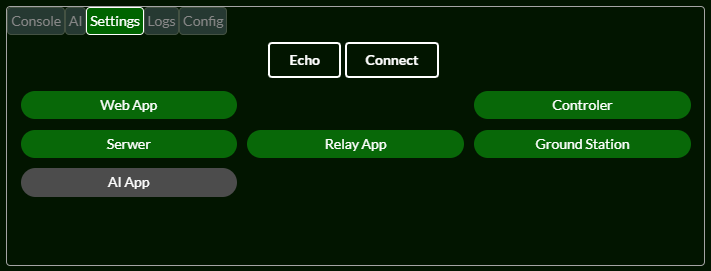
\includegraphics[width=1\textwidth]{settings}
    \caption{Dodać podpis :)}
\end{figure}


\paragraph{Strona: Odtwarzacz}\mbox{}

Strona odtwarzacza pozwala na podgląd zapisanych plików z danymi z przelotów (lista dostępnych plików znajduje się w zakładce Logs). Jest niezwykle istotna podczas analizy przelotów. Dostępne jest odtwarzanie i pauzowanie, przesuwanie pojedynczych klatek, dostosowanie prędkości odtwarzania (w zakresie od 0.1 do 10 razy) oraz przewijanie przy pomocy suwaka. Dodatkowo możliwe jest wyświetlanie wybranych danych na wykresie. Informacje z plików pokazywane są w formie wizualizacji oraz w zakładce z danymi w czasie rzeczywistym.

 \begin{figure}[H]
    \centering
    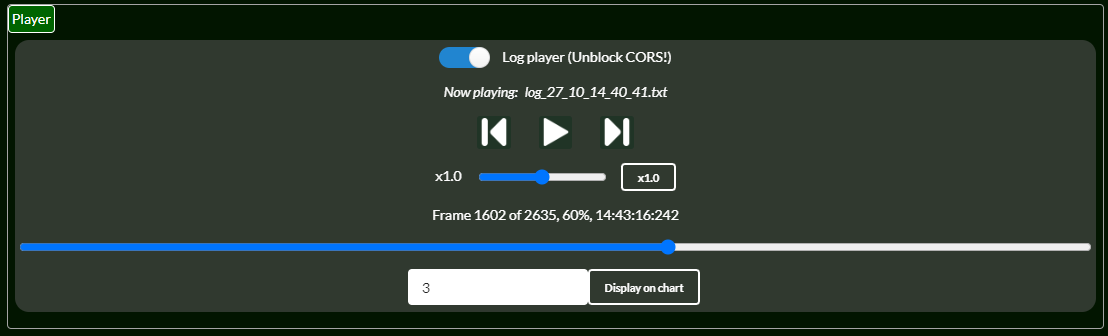
\includegraphics[width=1\textwidth]{player}
    \caption{Dodać podpis :)}
\end{figure}

\FloatBarrier
\subsection{Trening sieci neuronowej}
Zebranie danych potrzebnych do treningu i działania sieci wymagało przygotowania wszystkich elementów wymienionych w poprzednich rozdziałach. Sprawdzenie poprawności i niezawodności poszczególnych systemów i informacji okazało się kluczowe, ponieważ pozwoliło na zebranie poprawnych danych. 

W celu przygotowania algorytmów sztucznej inteligencji pierwszym krokiem było określenie wyboru algorytmu przetwarzania danych - wybór padł na rekurencyjną sieć neuronową, ze względu na sposób i możliwość jej nauczania, a także na możliwość brania pod uwagę poprzedniej chwili czasowej. Zgodnie z założeniem projektu, sterowanie samolotem ma się odbywać całkowicie w sposób sterowany przez sztuczną inteligencję - odpowiedź z sieci neuronowej jest kierowana prosto na serwomechanizmy i silnik. 

Kolejnym z założeń projektu było wykorzystanie doświadczenia pilotów w sterowaniu modelami samolotów bezpośrednio do nauki algorytmu sterowania. Lot modelem samolotu jest niezwykle trudnym zadaniem, a wykonanie wielu powtarzalnych przelotów trasy (w tym przypadku "ósemki") wymaga bardzo dużej ilości praktyki. Głównym pilotem samolotu został więc Kacper Krempa, wicemistrz Polski w kategorii lotów modelami F3K oraz wicemistrz Europy w lotach modeli kosmicznych.

Zadaniem sztucznej inteligencji jest więc zaobserwowanie stanu samolotu w powietrzu w locie manualnym oraz skorelowanie tego stanu z reakcją i zachowaniem pilota, poprzez odpowiednie wychyły drążków aparatury. Takie zachowanie powinno później zostać odtworzone podczas lotu autonomicznego. Aby określić stan samolotu, należy wziąć pod uwagę: wychylenie samolotu w osi roll oraz w osi pitch, te same wartości z poprzedniej chwili czasowej (różnica tych wartości może służyć stabilizacji), prędkość względem ziemi, wysokość względną od wysokości startu, prędkość względem powietrza, planowaną trajektorię lotu, a także rekurencyjną odpowiedź sieci z poprzedniej chwili czasowej. Warto zaznaczyć, że użyte serwomechanizmy są z rodziny serwomechanizmów analogowych, nie są one zatem w stanie wysłać informacji zwrotnej na temat rzeczywistego ustawienia. Przy małych różnicach w wychyleniu (rzędu kilkunastu stopni w ciągu sekundy) działania algorytmu możemy jednak uznać, że zadane ustawienie odpowiada rzeczywistemu.

 \begin{figure}[ht]
    \centering
    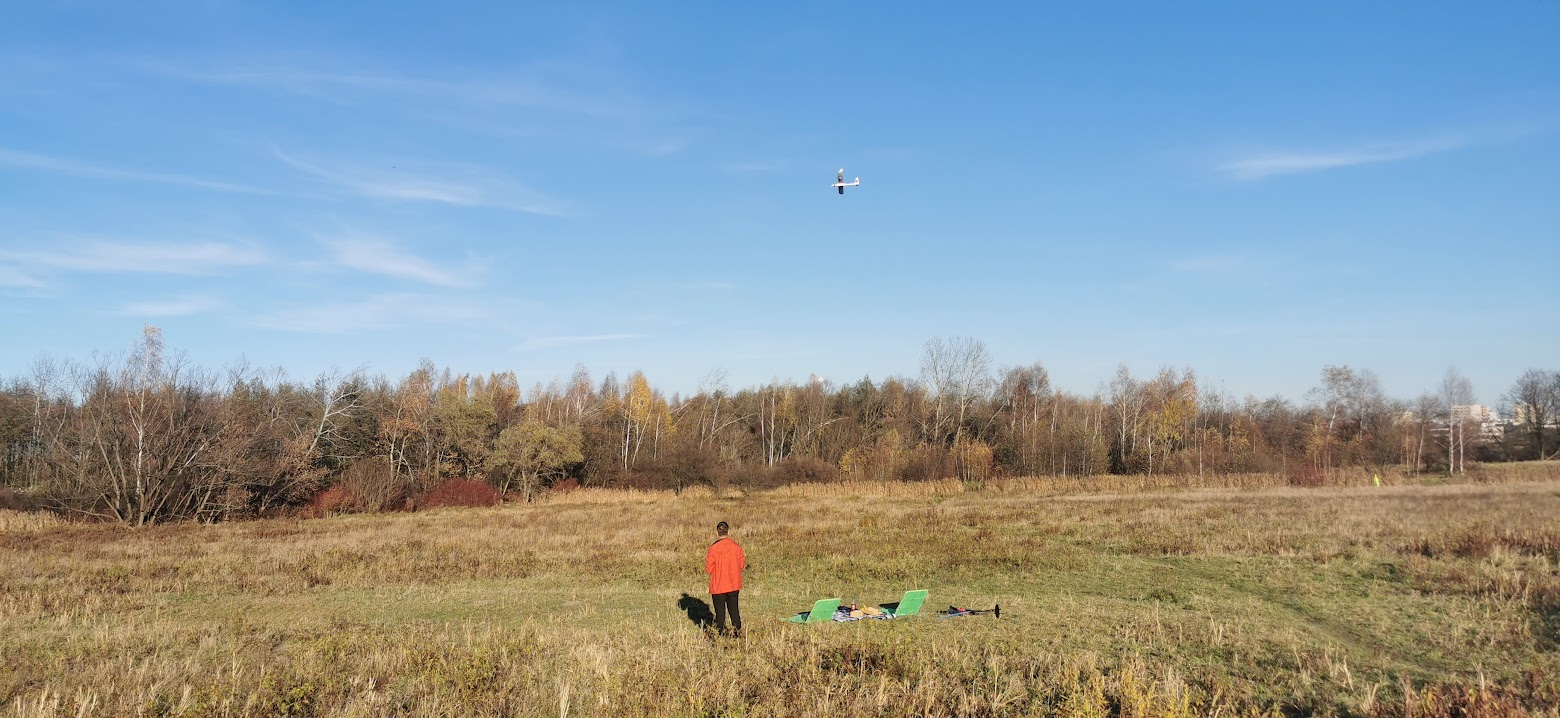
\includegraphics[width=1\textwidth]{kacperlata}
    \caption{Dodać podpis :)}
\end{figure}

Implementacja sieci i efektywny proces nauczania wymaga użycia biblioteki lub innego gotowego środowiska - przygotowanie i testowanie programów do treningu sieci przy pomocy algorytmów propagacji wstecznej jest bardzo czasochłonna i bezsensowna - istniejące rozwiązania okażą się prawdopodobnie bardziej sprawne i skuteczne. Dlatego po odrzuceniu początkowego pomysłu przygotowania własnego oprogramowania treningowego, zdecydowano się na użycie biblioteki TensorFlow w języku Python3. Umożliwia ona przygotowanie nawet bardzo złożonych algorytmów nauczania maszynowego, w tym także konwolucyjnych sieci neuronowych do przetwarzania obrazów, równocześnie korzystając z mocy obliczeniowej kart GPU. Poprawne zainstalowanie i konfiguracja jest dość uciążliwa, problematyczne jest zwłaszcza odpowiednia instalacja sterowników do karty graficznej, jednak po poprawnej instalacji dostępne jest bardzo wygodne środowisko do pracy ze sztuczną inteligencją. W systemie Windows do pracy z wirtualnym środowiskiem wykorzystano oprogramowanie Anakonda. Wykorzystana wersja Pythona to 3.7.9, natomiast wersja TensorFlow to 2.1. Użycie wyższych wersji Pythona nie jest możliwe ze względu na brak kompatybilności z drugą biblioteką.

Problem sterowania samolotem jest dość liniowy, wychylenie powietrzni sterowych związane jest w dość liniowy sposób z pozycją samolotu na trasie i może być wspomagany przez (również w dużym stopniu liniowy) problem stabilizacji. Dlatego wybrana sieć neuronowa nie jest głęboka - posiada 21 wejść, 10 neuronów ukrytych (w jednej warstwie), oraz 5 wyjść (4 serwomechanizmy oraz silnik).

 \begin{figure}[H]
    \centering
    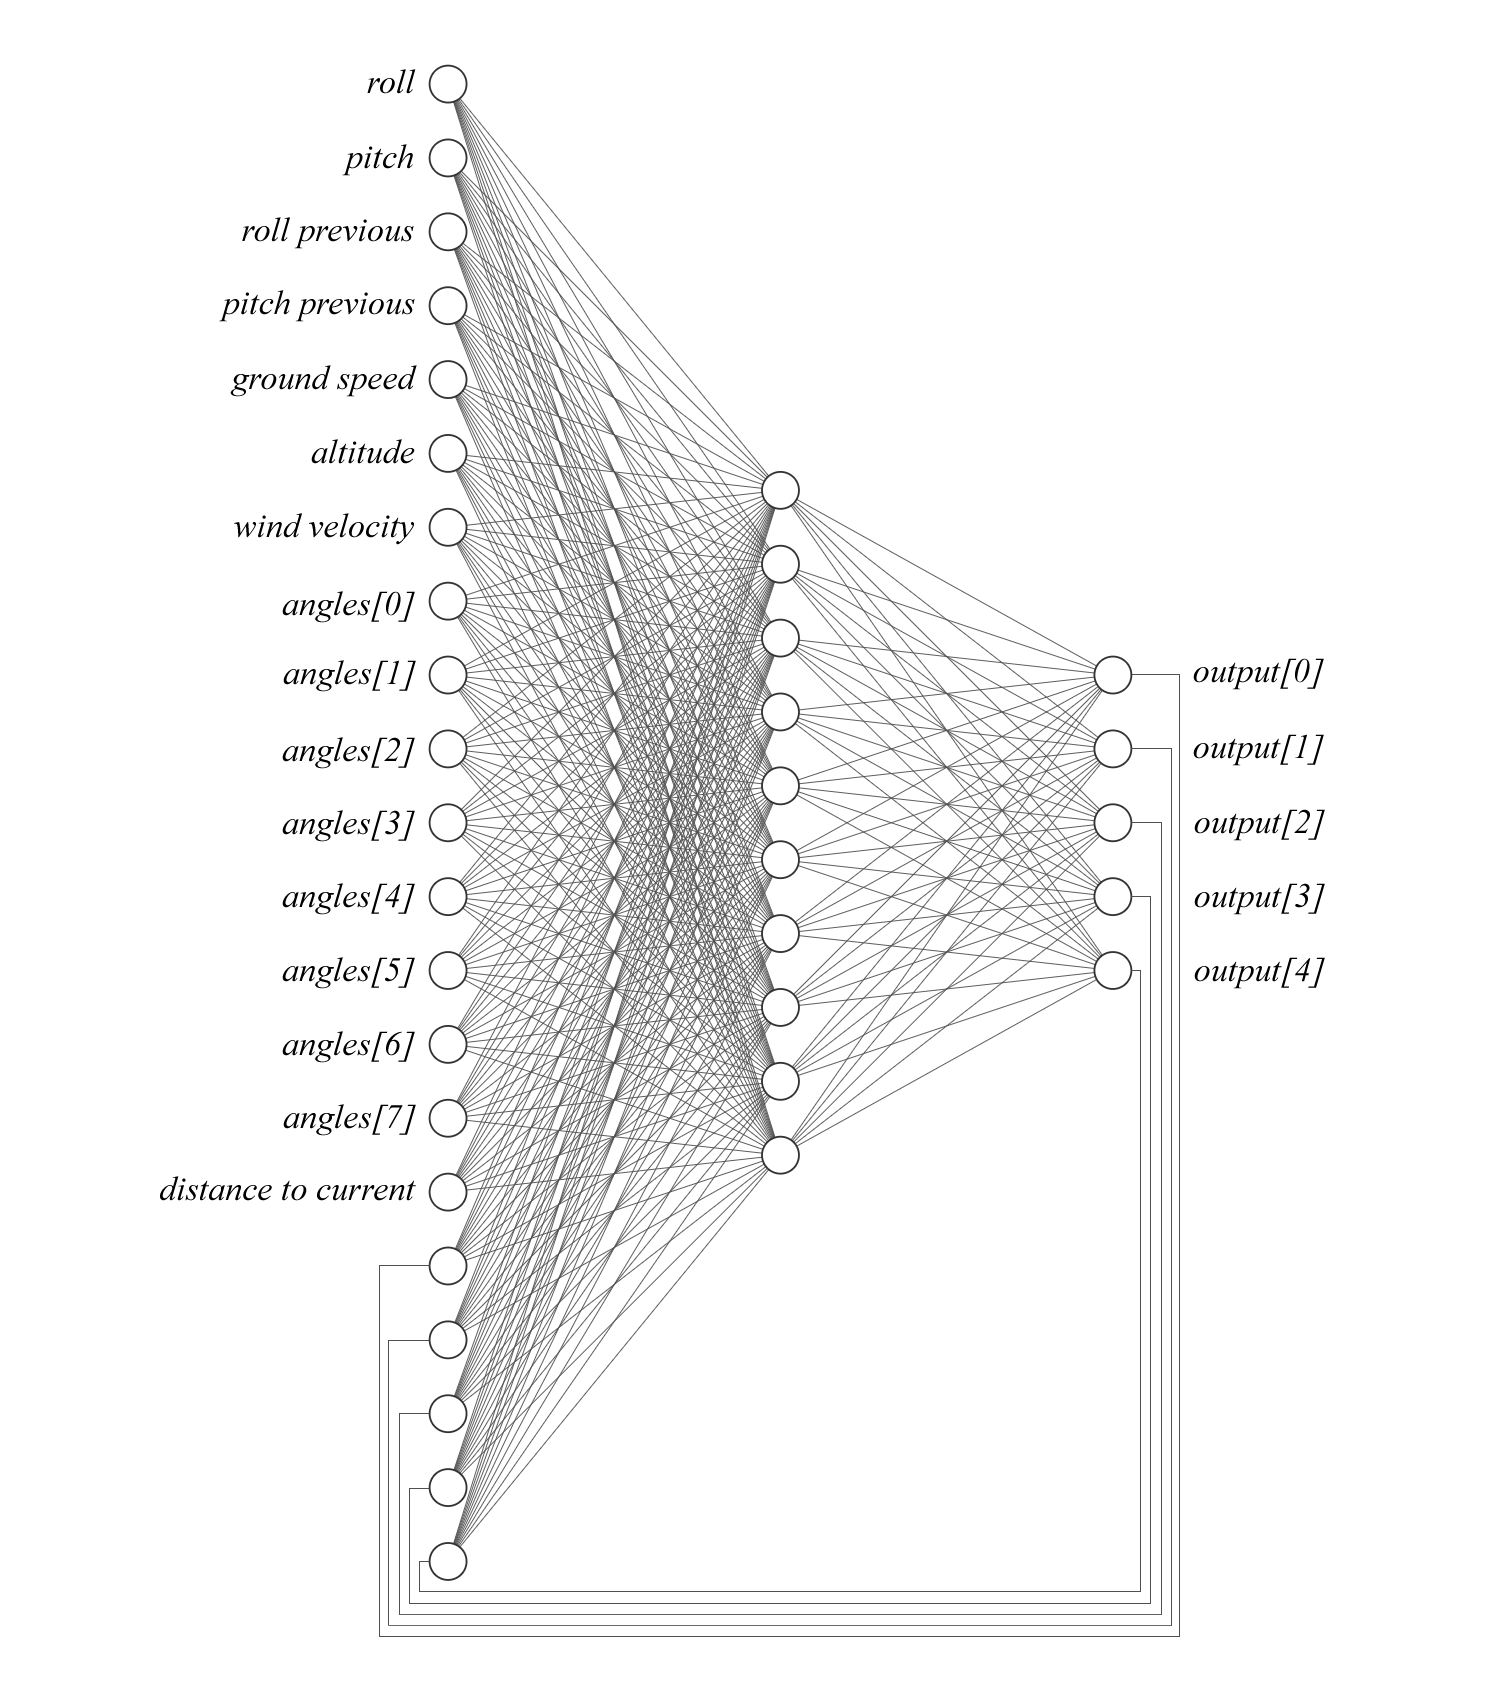
\includegraphics[width=1\textwidth]{siec}
    \caption{Dodać podpis :)}
\end{figure}

W bibliotece TensorFlow sieć ta zdefiniowana jest jako model typu Sequential, dodatkowo przyjęto sigmoidalną funkcję aktywacji oraz definicję błędu pomiarowego jako średni błąd kwadratowy. Do procesu nauczania wykorzystano dane zebrane podczas przelotów treningowych.


Trening został przeprowadzony na podstawie około 1500 chwil czasowych. Po około 35 epokach spadek błędu jest niewielki, dalsze działanie algorytmu może więc skutkować przeuczeniem sieci. Po przetestowaniu działania na przykładowych danych testowych otrzymany wynik predykcji sieci zdaje się być poprawny, zatem sieć można wstępnie uznać za wytrenowaną.

 \begin{figure}[H]
    \centering
    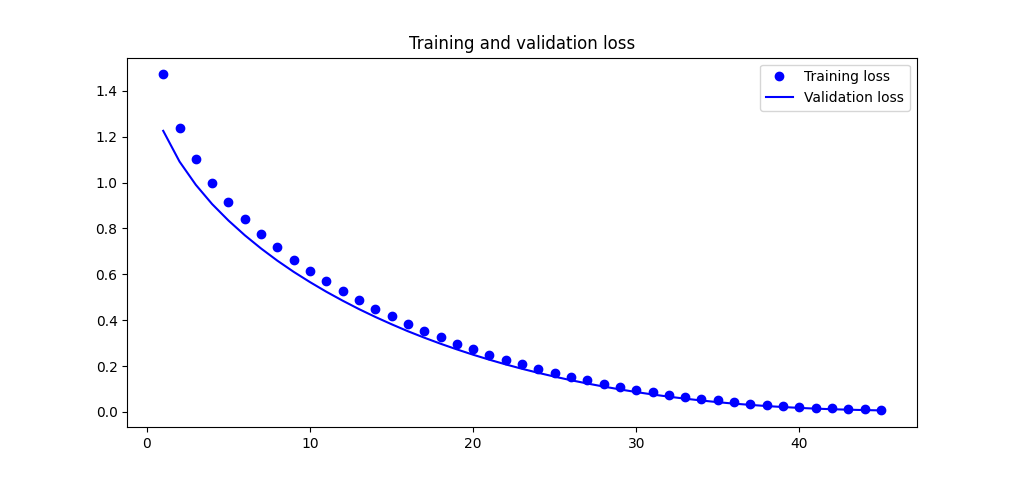
\includegraphics[width=1\textwidth]{tfloss}
    \caption{Dodać podpis :)}
\end{figure}

Jedną z wad biblioteki TensorFlow jest brak bezpośredniego dostępu do struktury wytrenowanej sieci neuronowej - macierzy wag połączeń oraz biasów. Sposobem na wygenerowanie modelu jest jego konwersja do pliku TFlite. Biblioteka TensorFlowLite jest biblioteką dedykowaną dla urządzeń mobilnych, która umożliwia na wykorzystanie modelu na docelowym urządzeniu, takim jak telefon, mikrokontroler czy w aplikacji komputerowej. Modele TFlite są lżejsze oraz zoptymalizowane do pracy z wykorzystaniem mniejszych zasobów obliczeniowych i pamięciowych.

Wersja biblioteki TensorFlowLite dostępna na mikrokontrolery jest kompatybilna ze środowiskiem Arduino IDE. Nie wspiera jednak ona sprzętowo wszytskich mikroprocesorów, oficjalnie wspierane jest niewiele urządzeń takich jak Arduino Nano 33 BLE Sense, STM32F746 czy ESP-EYE. Mimo braku oficjalnego wsparcia, na wykorzystanym w projekcie Teensy 4 z (mikroprocesor ARM Cortex-M7) istnieje możliwość uruchomienia biblioteki. Plik z modelem sieci neuronowej TFlite musi zostać zapisany przemieniony na tablicę, która może zostać zinterpretowana przez język C/C++. W tym celu można wykorzystać dostępną w systemach UNIX komendę xdd lub użyć skryptu w Pythonie. Finalnie otrzymany plik można zapisać z rozszerzeniem .h i zaimportować przez kompilator AVR-GCC po stronie środowiska Arduino. Model można poddać dodatkowemu procesowi kwantyzacji, co pozwala jeszcze bardziej ograniczyć jego zapotrzebowanie na moc obliczeniową oraz pamięciową. Podczas treningu liczby zmiennoprzecinkowe zapisane są w formacie float64, kwantyzacja pozwala na implementację z wykorzystaniem na przykład postaci float32 czy float16.

Niestety, przykładowych rozwiązań zastosowania modelu TensofFlow na mikrokontrolerach ze szczegółowym opisem ich implementacji jest w Internecie bardzo niewielka ilość, dokumentacja również jest skromna i nie zawiera opisu rozwiązań wielu problemów. To wszystko sprawiło, że praca z biblioteką okazała się bardzo uciążliwa. Po wielu próbach udało uruchomić wytrenowaną sieć, jednak problemem okazała się rozbieżność odpowiedzi sieci dla danych testowych w oryginalnej aplikacji uczącej i na mikrokontrolerze. Rozbieżność ta wynika najprawdopodobniej z konieczności skalowania danych wejściowych i wyjściowych (co jest częstą procedurą w implementacji tego typu sieci neuronowych), jednak próby naprawienia tego problemu nie powiodły się. 

Drugim równocześnie testowym oprogramowaniem do uczenia maszynowego było narzędzie Neural Net Fitting App z Deep Learning Toolbox w środowisku Matlab. Jego zdecydowaną przewagą nad biblioteką TensorFlow jest możliwość wyeksportowania macierzy wag i biasów wytrenowanej sieci neuronowej. Dodatkowo istnieje opcja wygenerowania źródłowego kodu do obsługi sieci w języku MATLAB. Dzięki temu przygotowany został skrypt umożliwiający konwersję wytrenowanego modelu - jego struktury i wartości - do pliku .h w języku C++. Na ten sam język przetłumaczone zostały funkcje odpowiadające za propagację sygnału przez sieć. Kolejnymi krokami algorytmu propagacji sieci są:

\begin{enumerate}
    \item Wpisane danych do macierzy wejściowej.
	\item Translacja wejścia o stały offset (odejmowanie).
	\item Skalowanie wejścia o stałą wzmocnienia (mnożenie).
	\item Translacja wejścia o wartość minimalną (dodawanie).
	\item Propagacja do drugiej warstwy:
	\begin{enumerate}
		\item Mnożenie macierzy wejściowej przez macierz wag połączeń.
		\item Translacja o bias.
		\item Transformacja funkcją tangensa hiperbolicznego.
	\end{enumerate}
	\item Analogiczna propagacja do warstwy wyjściowej.
	\item Translacja wyjścia o wartość minimalną (odejmowanie).
	\item Skalowanie wyjścia o stałą wzmocnienia (dzielenie).
	\item Translacja wyjścia o stały offset (dodawanie).
\end{enumerate}

Stałe skalowania i translacji są indywidualne dla każdego neuronu wejściowego i wyjściowego. Wykorzystany algorytm zwraca taką samą odpowiedź w środowisku treningowym (Matlab) jak i na mikrokontrolerze, osiągnięty zatem został cel implementacji zadanej sieci. 

Uwaga: przygotowany algorytm umożliwia automatyczną zmianę ilości neuronów w każdej z warstw, dopiero modyfikacja struktury sieci (ilości warstw ukrytych) wymagałaby ręcznej interwencji w oprogramowanie i powielenia propagacji między warstwami odpowiednią ilość razy.

\FloatBarrier

\subsection{Wyniki}

\section{Podsumowanie i wnioski}
\subsection{Podsumowanie wyników doświadczeń}
\subsection{Problemy}
\subsection{Możliwości rozwoju projektu}
\subsection{Wnioski}

\end{document}